\section{Data}\label{sec:background}

\subsection{Census sources and the definition of literacy}

The censuses of 1897, 1926 and 1939 define literacy in the same way. The census of 1897 recorded the ability to read. The census of 1926 recorded separately the ability to read, counted if the respondent could read at least by syllables, and the ability to write; in the published tables a literate person is one who can read, for comparability with 1897. The census of 1939 asked whether the respondent reads and writes, or only reads, in any language, and counted both as literate \citep{tssu1928,zhiromskaya1996}. The constancy of the definition removes the most obvious mechanical explanation of the gains between 1926 and 1939, and it implies that Arabic-script literacy among Muslim women was counted in 1897 and 1926.\footnote{The 1939 census is known to have been inflated in its population totals \citep{tolts2021,zhiromskaya2001,andreev1998}. The inflation was of the order of one to two per cent and concerned the count rather than the literacy question. Section~\ref{sec:robust2} shows that the literacy gains do not have the form a uniform inflation would produce.}

The 1926 census was taken on 17 December 1926 and the 1939 census on 17 January 1939, which is approximated by shifting the age window by twelve years; some respondents are thirteen years older. The census of 1897 was taken on 9 February, twenty-nine years and ten months before that of 1926, so that five-year age bands of 1897 correspond to five-year bands of 1926 shifted by thirty years. Volume 9 of the 1926 census recomputed the 1897 results to the 1927 borders of the nineteen Gosplan regions of the RSFSR, using the territorial coefficients of V.~P.~Efremov corrected by pre-war \emph{volost} populations; this official recomputation is the basis of the link from 1897 to 1926. Figure~\ref{fig:design} shows which birth cohorts are observed in which census and how old they were at the decree of 1919 and at the start of the cultural campaign in 1928.

\begin{figure}[htbp]\centering
\caption{Birth cohorts observed across the three censuses}\label{fig:design}
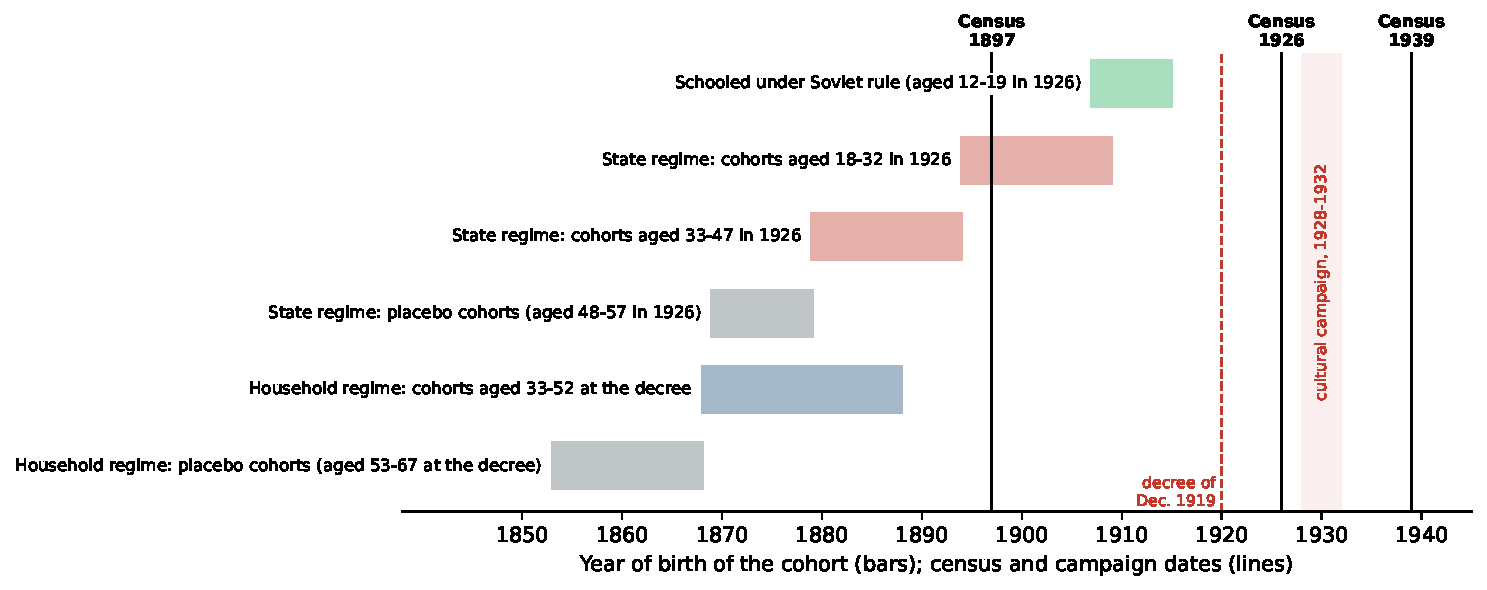
\includegraphics[width=0.95\linewidth]{fig01_design.pdf}
\note{Bars show the birth years of the cohorts used in the analysis; vertical lines mark the census dates; the dashed line marks the decree of December 1919 and the shaded band the cultural campaign of 1928 to 1932.}
\end{figure}

\subsection{The 1926 tables and their validation}

The regional volumes of the 1926 census print, for every \emph{guberniya}, \emph{okrug}, autonomous republic and autonomous oblast, a Table IX giving the population by single year of age, sex and literacy, for the whole population and for each of the most numerous nationalities, separately for the whole territory and for its urban and rural parts. These tables had not been digitised. From the scanned volumes held by the Russian State Library I transcribed Table IX for \N{d.units.distinct} territorial units, \N{d.cells} cells in all. Rural pages are available for \N{rus.units.rural} of them, and the analyses of the rural population use these. The units are eight autonomous units (the Tatar, Bashkir, Chuvash, Karelian and Volga German republics and the Mari, Votyak and Kalmyk autonomous oblasts), twenty Russian \emph{gubernii}, from Murmansk and Leningrad in the north-west through the Black Earth centre to Astrakhan and Orenburg in the south-east, and the sixteen \emph{okrugi} of the Ural oblast.

The tables carry the means of their own verification. Beside the single years of age they print a subtotal for every five years, so that each five-year figure exists twice, as the printed subtotal and as the sum of five single years transcribed separately. A five-year group enters the analysis if the two agree to within two persons or half of one per cent. Where they disagree, the figure is taken that satisfies one of two further identities of the table, that the urban and rural populations sum to the total and that the nationalities sum to the whole population. Where neither identity discriminates, the figure is taken that lies close to the two adjacent cohorts of the same series while the other does not. Groups that fail all three tests are dropped. Of the \N{d.g5} five-year groups between the ages of 10 and 69, \N{d.g5.t1} per cent pass the first test, \N{d.g5.t2} per cent the second and \N{d.g5.t3} per cent the third, and \N{d.g5.t0} per cent are dropped. The dropped groups include \N{d.g5.nbr} that pass the identities and differ from both adjacent cohorts by more than 25 points of literacy or by a factor of three in population, a pattern produced by an error that is present in both readings and that an identity cannot detect. Section~\ref{app:extract} describes the procedure in full. The validated data contain \N{d.bands} cells by unit, area, nationality, sex and age band, of which \N{d.bands.rural} are rural. Six units have rural pages on which fewer than 85 per cent of the single-year cells satisfy an identity (Astrakhan, Kungur, the Volga German republic, Orenburg, Penza and Samara); they are excluded in robustness checks.

\subsection{The linked cohorts}

Table XV of Volume 9 gives, for each of the nineteen Gosplan regions, the population by sex, five-year age band and literacy in 1926 and in 1897. Its \N{d.xv.cells} cells provide the linked cohorts of the household regime and, at the regional level, a replication of the state regime. Of the \N{d.xv.used} cells used, \N{d.xv.ok} satisfy the identity between the urban, rural and total figures. The 1939 tables of literacy by sex, age and urban or rural residence for every region of the RSFSR were declassified from the Russian State Archive of the Economy (fond 1562, opis' 336, dela 607 and 640) and digitised by Demoscope Weekly; I collected them for \N{d.c39.regions} regions (\N{d.c39.cells} cells). They are not by nationality. The table of the 1959 census that gives the population of the RSFSR by age, sex, level of education and literacy, separately for town and village (the same fond and opis', dela 1591 to 1594, also digitised by Demoscope Weekly), is used once, to check the 1939 figures on the same cohorts twenty years later.

A unit of 1926 can be linked to a successor of 1939 in 29 cases, of which 20 have rural pages. The cohorts of 1926 are built from validated single years of age, so that a cohort aged 18 to 22 in 1926 is compared with the group aged 30 to 34 in 1939. Four units whose successors of 1939 cannot be compared with them are excluded from every sample.\footnote{The Leningrad and Novgorod \emph{gubernii} were both absorbed into the Leningrad oblast of 1939, together with the Pskov \emph{guberniya}, so that the cohorts of 1939 are two to six times the size of those of 1926. The Nizhny Novgorod \emph{guberniya}, whose successor, the Gorky oblast, does not have its borders, and the Volga German republic have no rural pages in any case.} After validation, a cohort being used only where both of its sexes are validated, the rural sample of the state regime contains \N{w2.n} cells by unit, cohort and sex from \N{w2.units} units. The oblasts of 1939 do not have the borders of the \emph{gubernii} of 1926, and the Ural \emph{okrugi}, three of which are in the rural sample, are matched to the larger oblast that contained them. The comparison is between literacy rates, which a change of border affects only if the territory gained or lost differed in literacy, and Section~\ref{sec:robust2} repeats the analysis on the units whose cohorts changed in size by no more than mortality would imply, without the Ural \emph{okrugi}, and on the seventeen Gosplan regions that cover the whole RSFSR.

\subsection{Summary of the data}

Table~\ref{tab:data} lists the sources and the files built from them, Table~\ref{tab:sumstat} describes the three linked samples, and Table~\ref{tab:units} reports the transcription and the validation of every unit of 1926. Figure~\ref{fig:map} maps the units on the district boundaries of 1897.

\begin{table}[htbp]\centering
\caption{The data: sources, validated tables and linked samples}\label{tab:data}
\begingroup\small
\begin{tabular}{p{5.6cm}p{6.2cm}rr}
\toprule
Source or file & Content & Units & Cells \\
\midrule
\multicolumn{4}{l}{\textit{A. Sources}} \\
Census of 1926, Table IX of the regional volumes & Population by single year of age, sex, nationality and literacy, total, urban and rural & 44 & 90,642 \\
Census of 1926, Table XV of Volume 9 & Population by sex, age and literacy in 1926 and in 1897, borders of 1927 & 19 & 10,320 \\
Census of 1939 (RGAE, via Demoscope Weekly) & Population and illiterate by sex, age, urban and rural, by region & 75 & 12,144 \\
Census of 1959 (RGAE, via Demoscope Weekly) & Population by sex, age, education and literacy, RSFSR & 1 & 225 \\
\midrule
\multicolumn{4}{l}{\textit{B. Validated tables of 1926}} \\
Five-year groups, ages 10 to 69 & Unit, area, nationality, sex & & 8,840 \\
Single years of age, 8 to 57 & Unit, area, nationality, sex & & 37,596 \\
Age bands & Unit, area, nationality, sex & & 5,984 \\
\midrule
\multicolumn{4}{l}{\textit{C. Linked cohorts}} \\
1926 to 1939, units (main sample) & Rural, cohort by sex & 18 & 218 \\
1926 to 1939 and 1959, regions & Rural, cohort by sex & 17 & 238 \\
1897 to 1926, regions & Rural, cohort by sex & 19 & 265 \\
\bottomrule
\end{tabular}

\note{Cells are the figures of the source or the rows of the file built from it. RGAE is the Russian State Archive of the Economy (fond 1562, opis' 336).}
\endgroup
\end{table}

\begin{table}[htbp]\centering
\caption{Summary statistics of the linked samples, rural population}\label{tab:sumstat}
\begingroup\small
\fitwidth{\begin{tabular}{llrrrrrrr}
\toprule
 & & & \multicolumn{2}{c}{Literate, per cent} & \multicolumn{3}{c}{Change, points} & Survival \\
\cmidrule(lr){4-5}\cmidrule(lr){6-8}
Sample & Sex & Cells & earlier & later & mean & SD & range & ratio \\
\midrule
1926 to 1939, units & women & 109 & 24.0 & 39.0 & 15.0 & 9.7 & 1 to 37 & 0.85 \\
 & men & 109 & 67.7 & 76.5 & 8.9 & 6.1 & $-$5 to 29 & 0.76 \\
1926 to 1939, regions & women & 119 & 24.2 & 37.3 & 13.1 & 9.8 & 1 to 55 & 0.75 \\
 & men & 119 & 63.9 & 74.2 & 10.3 & 10.7 & 0 to 54 & 0.66 \\
1897 to 1926, regions & women & 132 & 8.9 & 7.9 & $-$1.0 & 2.6 & $-$8 to 7 & 0.53 \\
 & men & 133 & 32.0 & 38.2 & 6.2 & 9.9 & $-$10 to 36 & 0.47 \\
\bottomrule
\end{tabular}
}
\note{Unweighted means over the cells of each sample, all cohorts including those above the age limit. A cell is a cohort of one sex in one unit or region. The survival ratio is the median of the number of the cohort at the later census divided by its number at the earlier census.}
\endgroup
\end{table}

\begin{figure}[htbp]\centering
\caption{The units of the 1926 tables: women's literacy and the gender gap at ages 20 to 24, rural, 1926}\label{fig:map}
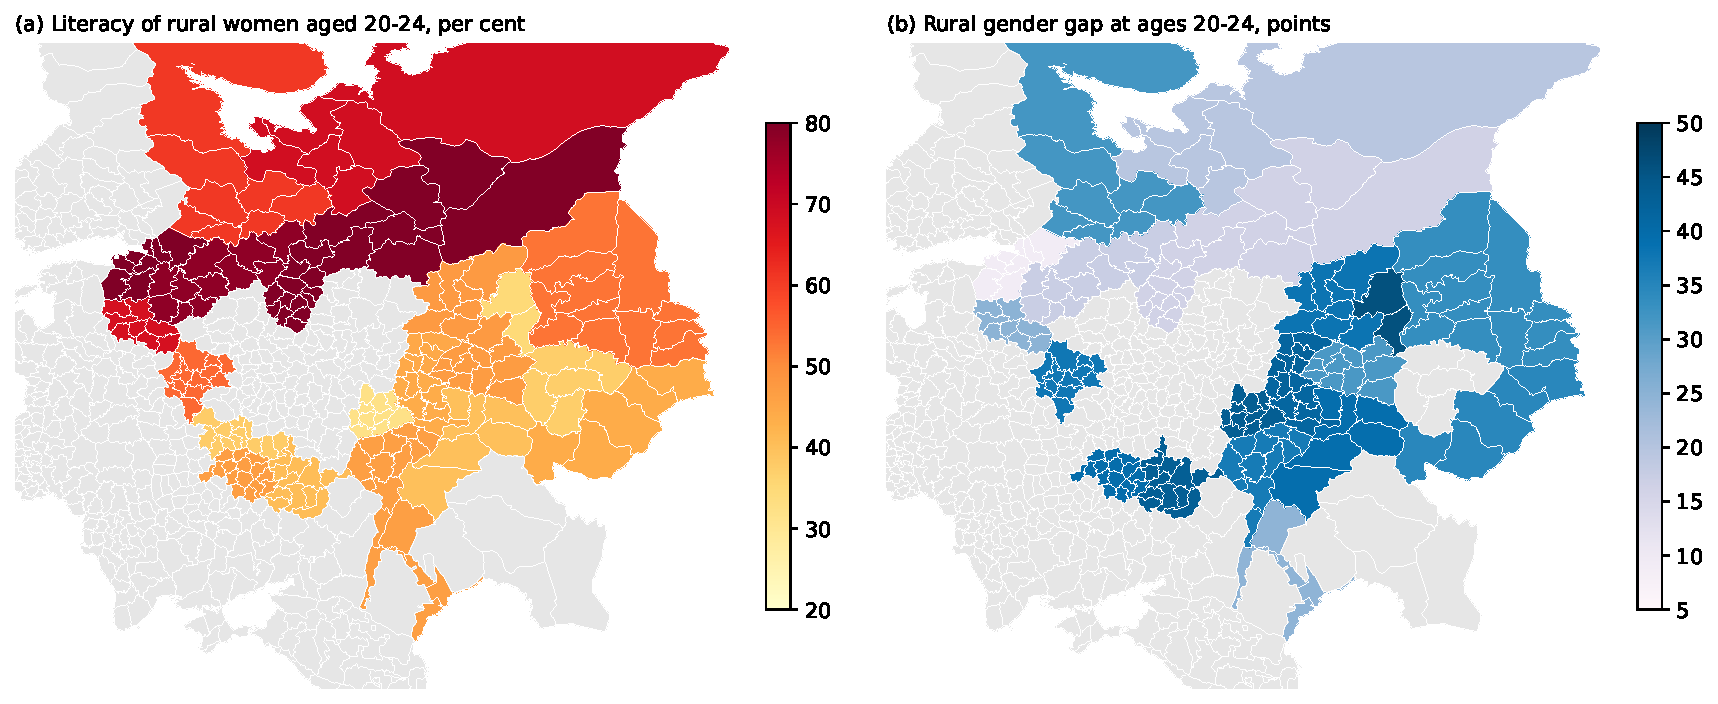
\includegraphics[width=\linewidth]{fig22_map_1926.pdf}
\note{District boundaries of 1897 from \citet{malein2023}; districts are coloured by the value of the 1926 unit to which they belong (provinces divided between several units carry the mean of those units). Grey districts are outside the sample or have no validated cell. Panel (a): literacy of rural women aged 20 to 24, all nationalities; panel (b): male minus female literacy at the same ages.}
\end{figure}

Figure~\ref{fig:profile} shows the age and sex profile of rural literacy in 1926 pooled over the units. Men's literacy peaks at \N{prof.M.20-24} per cent in the cohorts aged 20 to 29, who were of school age before 1917 and of conscription age during the wars; women's peaks at \N{prof.F.20-24} per cent at ages 20 to 24 and falls to \N{prof.F.40-49} per cent at ages 40 to 49. The gender gap is \N{prof.gap.8-11} points among children aged 8 to 11, \N{prof.gap.20-24} points at 20 to 24 and \N{prof.gap.30-39} points at 30 to 39.

\begin{figure}[htbp]\centering
\caption{Literacy by age and sex in the 1926 census, rural population}\label{fig:profile}
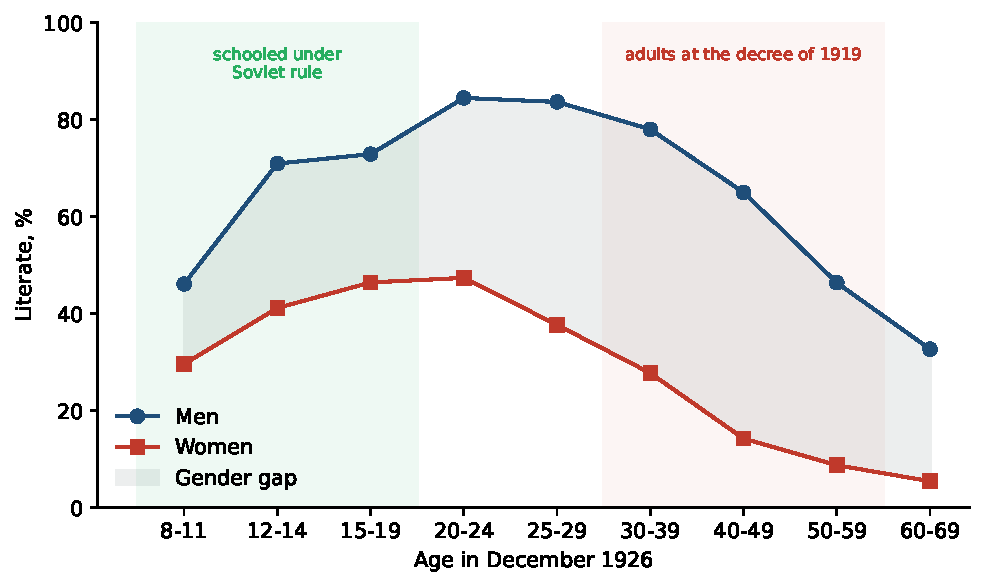
\includegraphics[width=0.85\linewidth]{fig02_age_profile_1926.pdf}
\note{Population-weighted over the units with validated rural cells, all nationalities. The green band marks cohorts schooled entirely under Soviet rule and the red band cohorts that were adults at the decree of 1919.}
\end{figure}

\FloatBarrier
\subsection{Transcription and validation of the 1926 tables}\label{app:extract}

The tables were transcribed by hand from the scans of the regional volumes held by the Russian State Library, page by page, into a spreadsheet with one row per single year of age and one column per nationality, sex and literacy status. The transcription was then checked in two ways. First, an automatic reading of every page was obtained with a neural recogniser, and each hand-entered cell was compared with the machine reading of the same cell. Cells on which the two disagreed were re-examined against the scan. Second, every figure was tested against the arithmetic of the tables themselves, in the following order.

Figure~\ref{fig:scan} shows a page of the source. Each page gives, for one unit and one area, the population and the literate by single year of age and sex for the whole population and for each nationality, and every fifth row, printed in bold, is the subtotal of the five-year group above it.

\begin{figure}[htbp]\centering
\caption{A page of Table IX of the census of 1926: the Tatar republic, rural areas}\label{fig:scan}
\begin{minipage}[b]{0.56\linewidth}\centering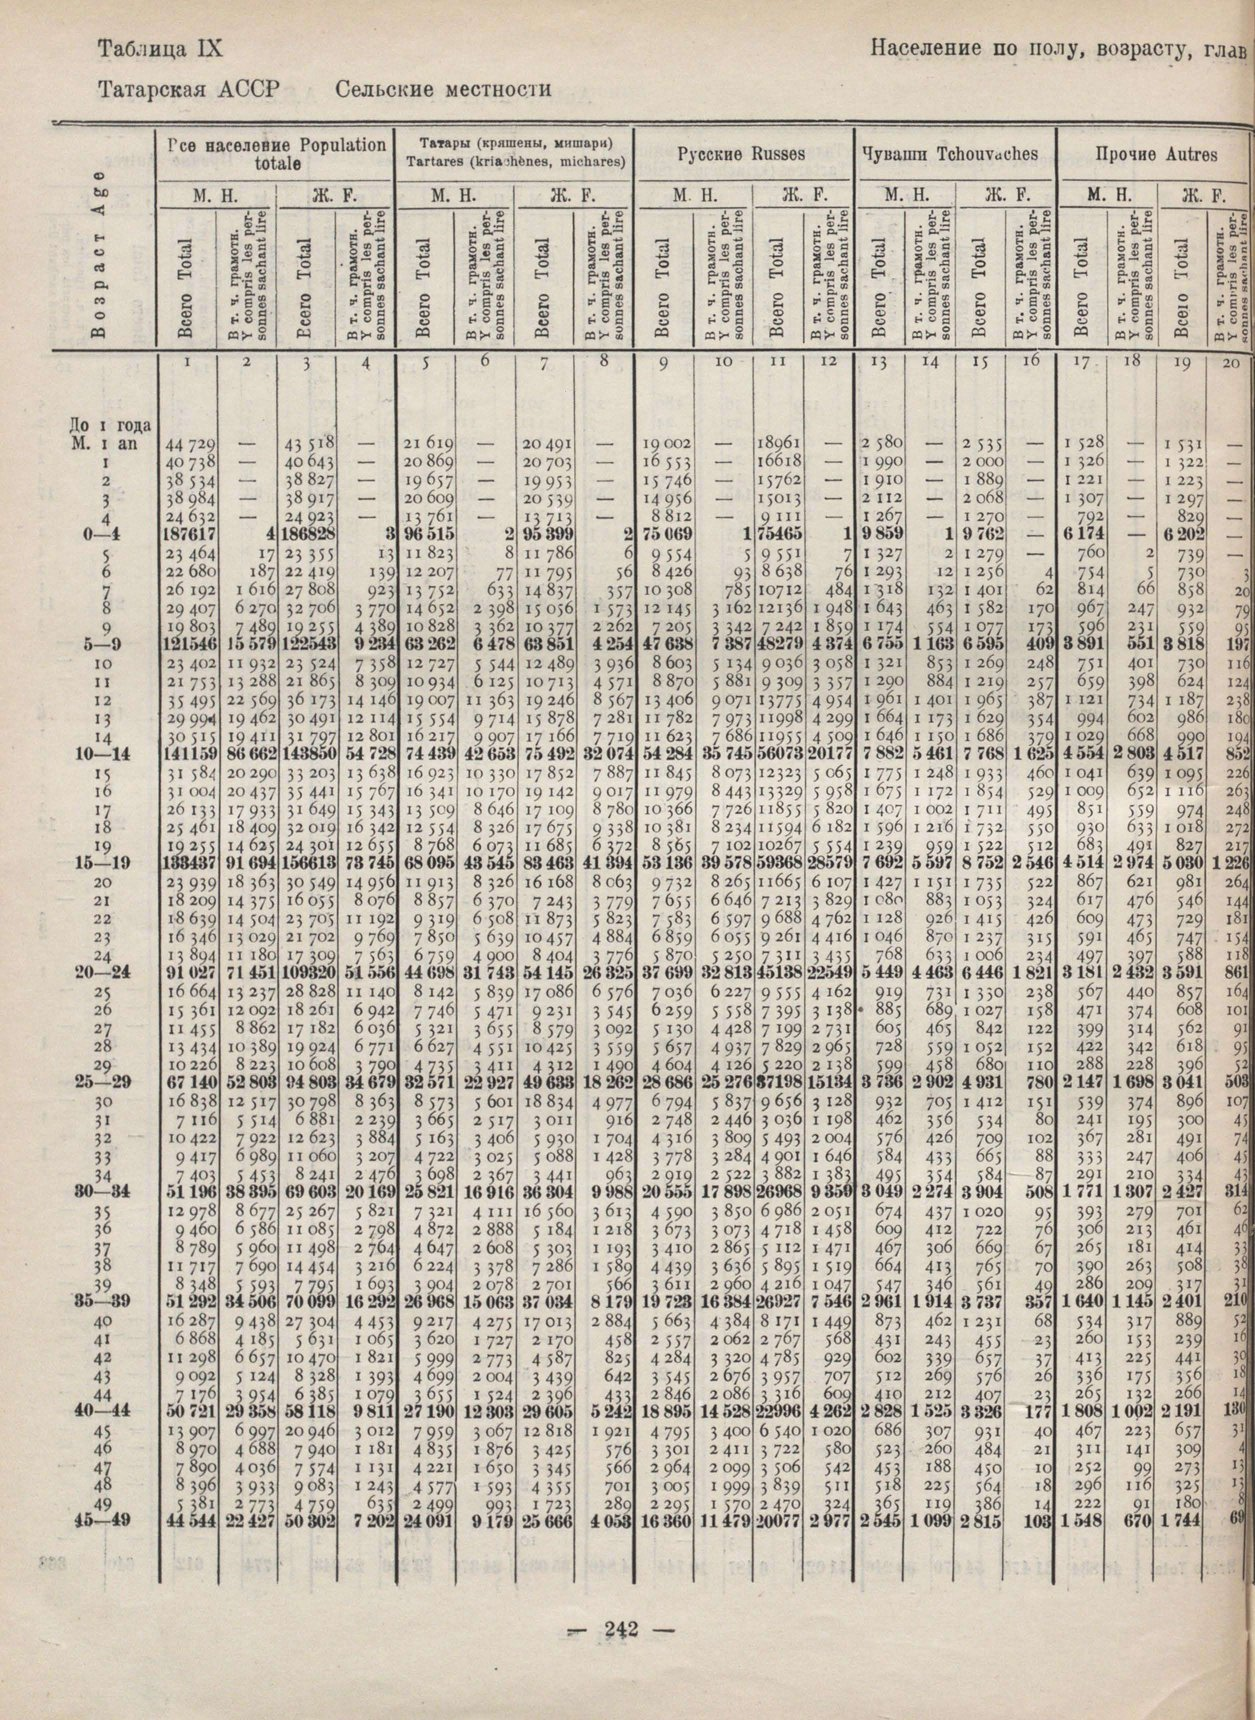
\includegraphics[width=\linewidth]{scan_tableIX_tatar_rural_p242.jpg}\\[2pt]\footnotesize (a) The page\end{minipage}\hfill
\begin{minipage}[b]{0.41\linewidth}\centering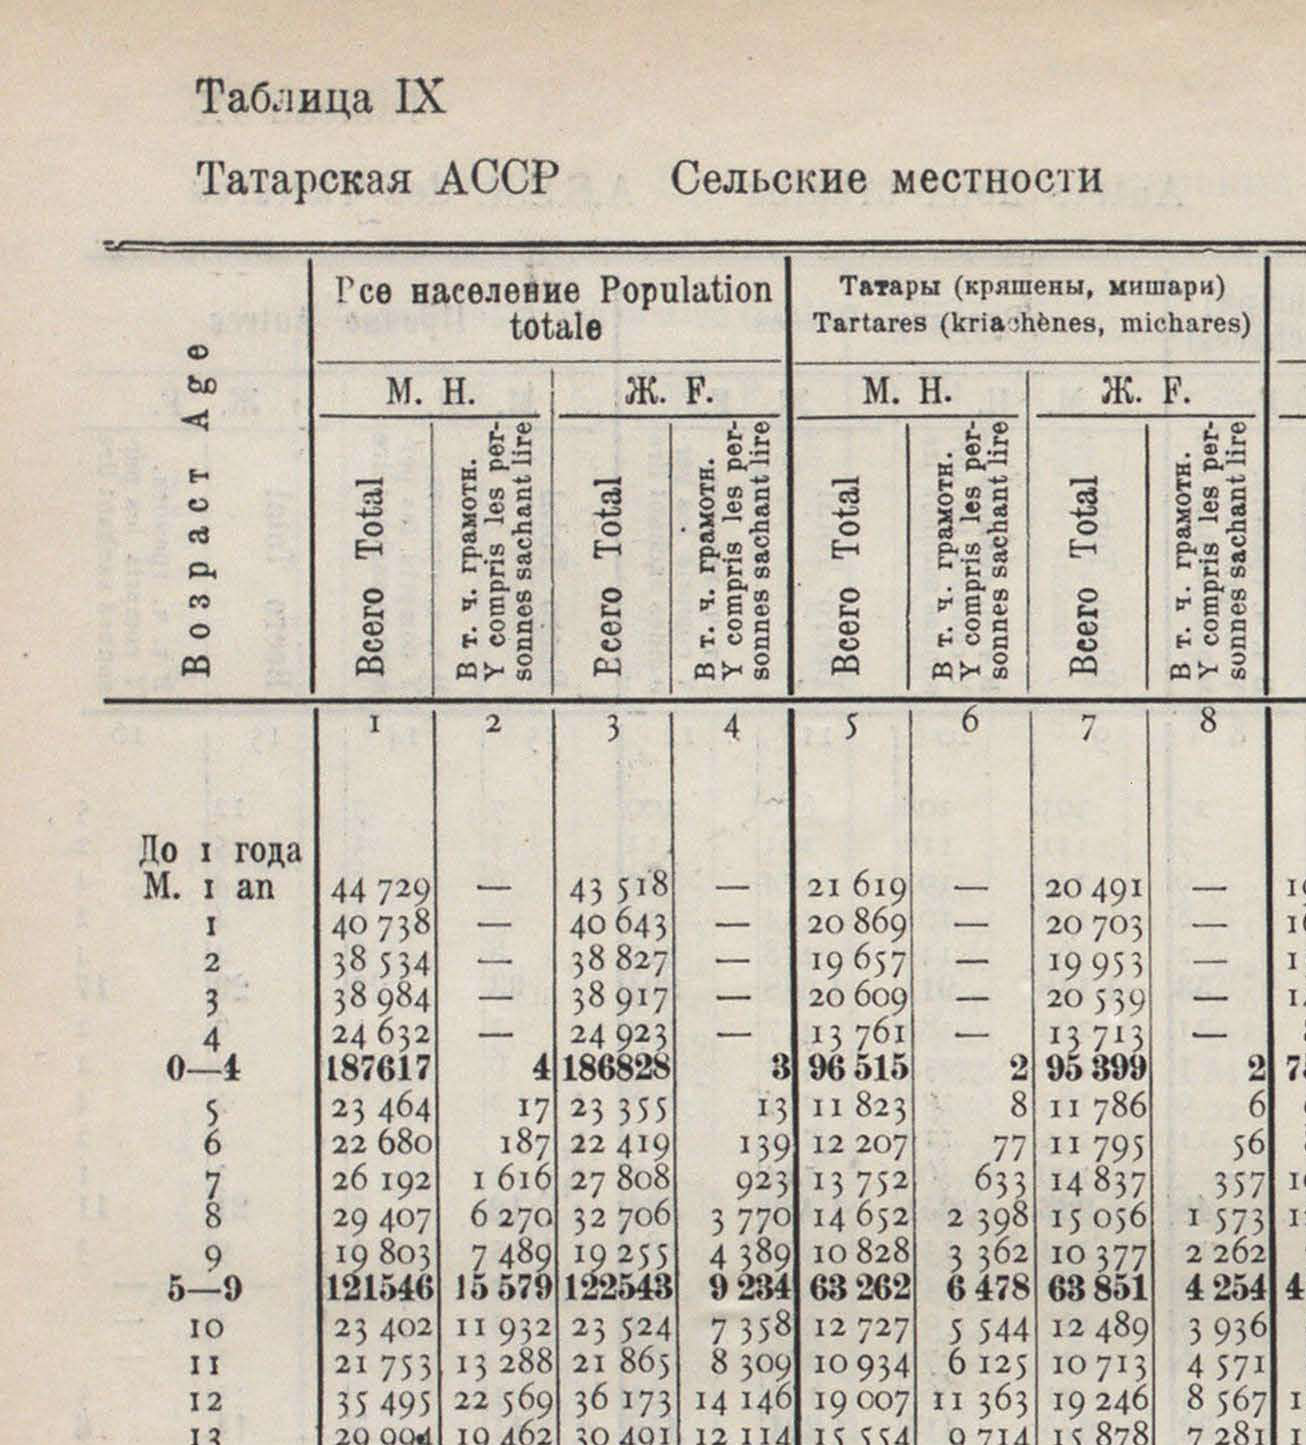
\includegraphics[width=\linewidth]{scan_tableIX_tatar_rural_p242_detail.png}\\[2pt]\footnotesize (b) Detail, ages 0 to 14\end{minipage}
\note{Volume 3 of the census of 1926, page 242, from the scan of the Russian State Library. The rows 0--4, 5--9 and 10--14 in bold are the printed subtotals against which the sums of the single years are checked.}
\end{figure}

\emph{The printed subtotal.} Table IX prints, after every five single years of age, the subtotal of the five-year group. For each unit, area (total, urban or rural), nationality and sex, and separately for the population and for the literate, the printed subtotal $P$ is compared with the sum $S$ of the five single years. If they agree to within two persons or half of one per cent, the group is validated by the first test.

\emph{The identities of the table.} If $P$ and $S$ disagree, or one of them is illegible, two further identities are used, computed from groups that have passed the first test. The urban and rural figures must sum to the total, and the nationalities must sum to the whole population. If exactly one of $P$ and $S$ satisfies an identity, it is taken. If both are missing and the two identities agree with each other, their value is taken.

\emph{The adjacent cohorts.} If no identity discriminates, $P$ and $S$ are compared with the mean of the two adjacent five-year groups of the same series. The one is taken that lies within 15 points of literacy of that mean, or within 40 per cent of it for the population, provided that the other does not.

A group that fails the three tests is dropped. A single year of age is used only if its five-year group has been validated and the validated figure is the sum of the single years. An error that was made in the printed subtotal and in a single year alike, as happens when a digit of the printed page is misread consistently, passes every identity. A last rule therefore drops the groups of at least 100 persons whose literacy differs by more than 25 points from both adjacent groups, and those whose population is more than three times, or less than a third of, both adjacent groups. The age bands used in the analysis are sums of validated groups, or of validated single years for the bands 8 to 11 and 12 to 14 and for the cohorts linked to 1939. Bands with fewer than 200 persons, series with fewer than three bands, and bands that differ by more than 30 points from both adjacent bands are dropped.

Of the \N{d.g5} five-year groups between the ages of 10 and 69, \N{d.g5.t1} per cent are validated by the first test, \N{d.g5.t2} per cent by the second and \N{d.g5.t3} per cent by the third. In the rural population the shares are \N{d.g5r.t1}, \N{d.g5r.t2} and \N{d.g5r.t3} per cent of \N{d.g5r} groups. Of the \N{d.single} single-year cells between the ages of 8 and 57, \N{d.single.valid} per cent are validated. The results of the paper are unchanged when only the figures validated by the first two tests are used (Table~\ref{tab:a2}). Figure~\ref{fig:heat} shows the literacy of rural women by unit and cohort in the validated data.

\begin{figure}[htbp]\centering
\caption{Women's literacy by unit and cohort, rural, 1926}\label{fig:heat}
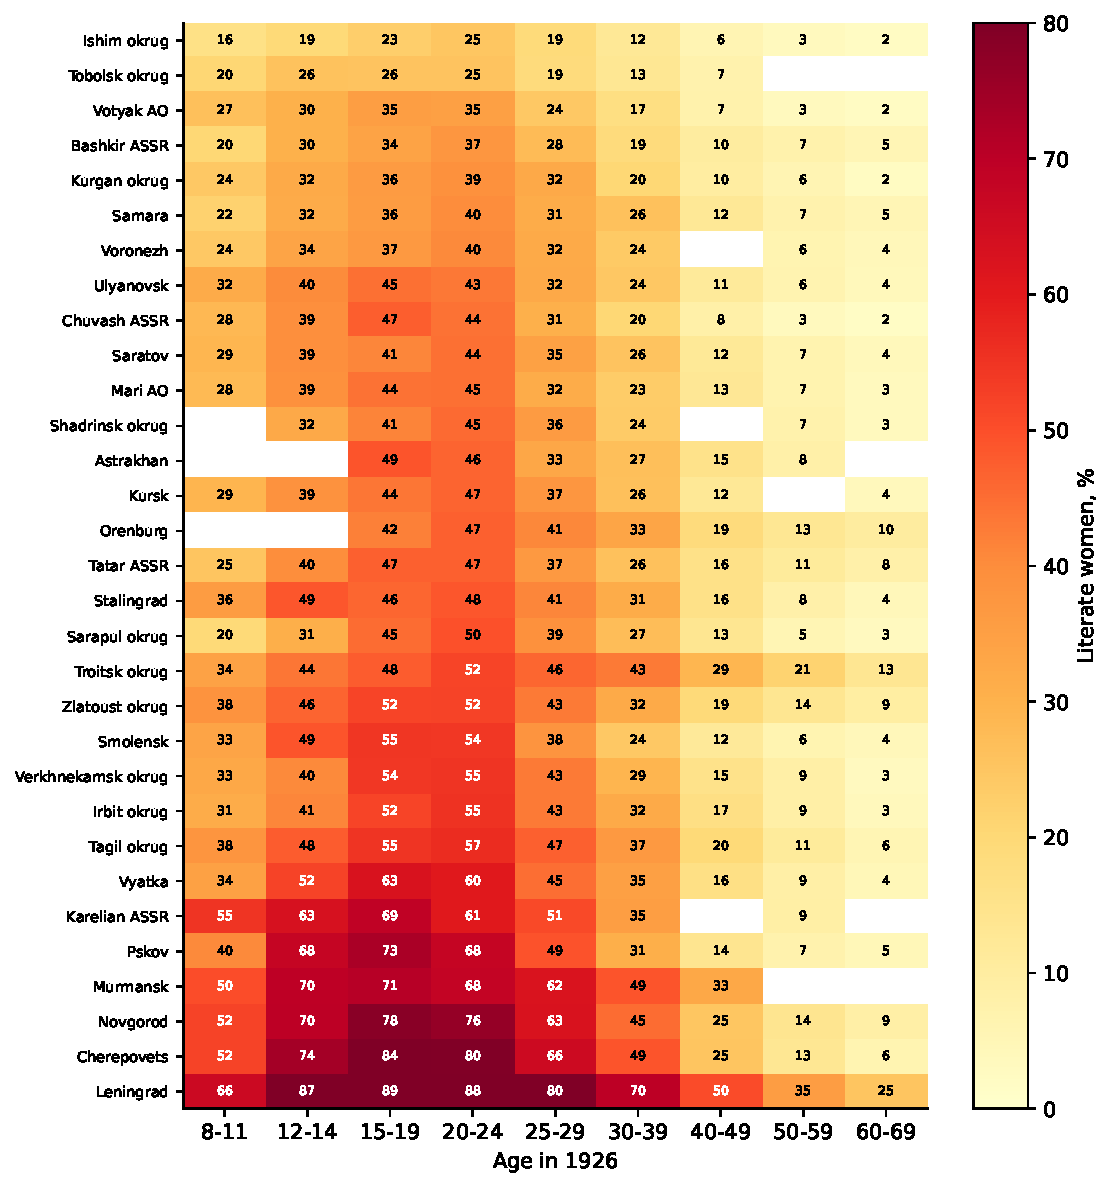
\includegraphics[width=0.8\linewidth]{fig12_heatmap_women_1926.pdf}
\note{All nationalities, validated cells; blank cells did not pass validation. Units with validated cells in the four bands between the ages of 15 and 39.}
\end{figure}

\begin{table}[htbp]\centering
\caption{The units of Table IX of the census of 1926: transcription and validation}\label{tab:units}
\begingroup\footnotesize\setstretch{1.0}\renewcommand{\arraystretch}{0.86}
\begin{tabular}{lrrcrrrc}
\toprule
 & Cells & Nation- & Rural & Five-year & \multicolumn{2}{c}{Validated, per cent} & Main \\
\cmidrule(lr){6-7}
Unit & transcribed & alities & pages & groups & first test & all tests & sample \\
\midrule
\multicolumn{8}{l}{\textit{Autonomous republics}} \\
Bashkir ASSR & 4,428 & 8 & yes & 432 & 98.4 & 98.8 & $\bullet$ \\
Chuvash ASSR & 1,968 & 3 & yes & 192 & 99.5 & 100.0 & $\bullet$ \\
Karelian ASSR & 1,968 & 3 & yes & 192 & 95.8 & 95.8 & $\bullet$ \\
Tatar ASSR & 2,460 & 4 & yes & 240 & 100.0 & 100.0 & $\bullet$ \\
Volga German ASSR & 1,830 & 4 & yes & 200 & 73.0 & 78.0 &  \\
\multicolumn{8}{l}{\textit{Autonomous oblasts}} \\
Kalmyk AO & 360 & 2 & -- & 48 & 97.9 & 100.0 &  \\
Mari AO & 1,968 & 3 & yes & 192 & 94.8 & 94.8 & $\bullet$ \\
Votyak AO & 1,968 & 3 & yes & 192 & 97.4 & 99.5 & $\bullet$ \\
\multicolumn{8}{l}{\textit{\emph{Gubernii}}} \\
Astrakhan & 1,830 & 4 & yes & 200 & 75.0 & 78.0 &  \\
Bryansk & 2,460 & 4 & yes & 240 & 78.3 & 80.8 &  \\
Cherepovets & 2,214 & 2 & yes & 216 & 100.0 & 100.0 &  \\
Kursk & 1,968 & 3 & yes & 192 & 96.9 & 97.4 & $\bullet$ \\
Leningrad & 2,952 & 3 & yes & 96 & 96.9 & 99.0 &  \\
Murmansk & 1,080 & 2 & yes & 144 & 100.0 & 100.0 &  \\
Nizhny Novgorod & 1,230 & 4 & -- & 120 & 76.7 & 76.7 &  \\
Novgorod & 2,214 & 2 & yes & 216 & 97.7 & 99.5 &  \\
Orel & 738 & 2 & -- & 72 & 100.0 & 100.0 &  \\
Orenburg & 2,460 & 4 & yes & 240 & 85.0 & 86.2 & $\bullet$ \\
Penza & 2,460 & 4 & yes & 240 & 83.8 & 87.5 & $\bullet$ \\
Pskov & 2,214 & 2 & yes & 216 & 98.1 & 100.0 &  \\
Samara & 3,444 & 6 & yes & 336 & 81.8 & 83.6 & $\bullet$ \\
Saratov & 3,444 & 6 & yes & 336 & 98.2 & 99.1 & $\bullet$ \\
Smolensk & 1,968 & 3 & yes & 192 & 89.1 & 93.2 & $\bullet$ \\
Stalingrad & 1,968 & 3 & yes & 192 & 97.9 & 98.4 & $\bullet$ \\
Tambov & 738 & 2 & -- & 72 & 94.4 & 97.2 &  \\
Ulyanovsk & 2,196 & 5 & yes & 240 & 97.9 & 99.2 &  \\
Voronezh & 1,968 & 3 & yes & 192 & 90.1 & 93.8 & $\bullet$ \\
Vyatka & 1,968 & 3 & yes & 192 & 97.9 & 99.0 & $\bullet$ \\
\multicolumn{8}{l}{\textit{\emph{Okrugi} of the Ural oblast}} \\
Chelyabinsk okrug & 984 & 3 & -- & 96 & 96.9 & 97.9 &  \\
Irbit okrug & 2,952 & 3 & yes & 288 & 85.4 & 92.0 &  \\
Ishim okrug & 2,952 & 3 & yes & 288 & 92.0 & 97.2 & $\bullet$ \\
Komi-Permyak okrug & 984 & 3 & -- & 96 & 82.3 & 83.3 &  \\
Kungur okrug & 1,968 & 3 & yes & 192 & 93.2 & 93.2 &  \\
Kurgan okrug & 2,952 & 3 & yes & 288 & 95.1 & 96.5 & $\bullet$ \\
Perm okrug & 984 & 3 & -- & 96 & 89.6 & 92.7 &  \\
Sarapul okrug & 1,968 & 3 & yes & 192 & 83.3 & 83.3 &  \\
Shadrinsk okrug & 2,952 & 3 & yes & 288 & 87.8 & 91.3 &  \\
Sverdlovsk okrug & 480 & 3 & -- & 64 & 100.0 & 100.0 &  \\
Tagil okrug & 1,968 & 3 & yes & 192 & 97.9 & 97.9 &  \\
Tobolsk okrug & 1,440 & 3 & yes & 192 & 92.2 & 97.9 & $\bullet$ \\
Troitsk okrug & 1,968 & 3 & yes & 192 & 97.9 & 99.0 &  \\
Tyumen okrug & 984 & 3 & -- & 96 & 96.9 & 97.9 &  \\
Verkhnekamsk okrug & 2,952 & 3 & yes & 288 & 93.8 & 95.8 &  \\
Zlatoust okrug & 2,952 & 3 & yes & 288 & 79.5 & 82.3 &  \\
\midrule
All 44 units & 89,904 & & 35 & 8,768 & 91.7 & 93.6 & 18 \\
\bottomrule
\end{tabular}

\note{Cells transcribed are all figures of the unit, for the whole territory and for its urban and rural parts. Nationalities are the groups printed in the table, including the group of other nationalities. Five-year groups are those between the ages of 10 and 69 by area, nationality and sex, and the validated shares are those passing the first test and any of the three tests. The main sample marks the units linked to 1939 with validated rural pages. The table of the Ural oblast as a whole, the sum of its \emph{okrugi}, was transcribed as a check and is not shown.}
\endgroup
\end{table}

\FloatBarrier
\section{A Model of Household and State Investment in Literacy}\label{sec:model}

The model states the conditions under which a household and a state teach an adult to read, and derives from the difference between them the predictions tested in Section~\ref{sec:why}.

\subsection{The household}

A household consists of members indexed by sex $s\in\{m,f\}$ and age $a$. Teaching a member to read costs $c$ in foregone labour and effort, and teaching a woman costs in addition $\phi n$, the care of the $n$ young children of the household that she would forgo. A literate member of sex $s$ earns a private return $r_s$ per period from age $a$ until the end of working life $T$. The household discounts at rate $\rho$, so that the present value of the private return is $r_s A(T-a)$, where $A(x)=\sum_{t=1}^{x}(1+\rho)^{-t}$. A literate woman also raises the human capital of her children, worth $\gamma$. The household values this only through altruism $\alpha<1$ and receives it a generation later, after $\tau$ periods. The household teaches member $(s,a)$ if
\begin{equation}\label{eq:hh}
  V_s(a,n)\;\equiv\; r_s\,A(T-a) \;+\; \mathbf{1}\{s=f\}\left[\frac{\alpha\gamma}{(1+\rho)^{\tau}}-\phi n\right] \;\ge\; c .
\end{equation}
This is the condition of \citet{benporath1967} with a sex-specific return, a discounted intergenerational term and a cost of time. The household is treated as a single decision-maker. If the decision belongs to its head, his valuation of the literacy of a wife or a daughter takes the place of the term in brackets and the condition keeps its form \citep{doepke2009}. Instruction that reaches a member outside the household and at no cost to it, as the army's reached the conscript, enters as a lower $c$ for sons. Let the cost $c$ vary across households with distribution function $H$. The share of members of sex $s$ and age $a$ who are taught is then $H\big(V_s(a,n)\big)$.

Three properties follow. First, the share taught declines with age for each sex, since $A(T-a)$ falls in $a$, and for men it declines from a high level, since $r_m$ is large. Second, when $r_f$ is close to zero, as it was for rural women whose labour was on the family plot, $V_f$ has no private-return age gradient only when fertility, child benefits, opportunity costs and the cost distribution are also held fixed. Low private returns alone do not imply zero learning or an age-invariant female profile. Third, anything that raises the private return $r_f$, such as the prospect of promotion that literacy opened in the 1930s, raises the share of women taught by the household, and raises it most where the return rises most. This is the incentive explanation of Section~\ref{sec:why}.

\subsection{The state}

The state values the same literacy at its social return. This comprises the private return, the intergenerational return $\gamma$ undiscounted by altruism and by the generation of delay, and a political return $\pi$ from a reading citizen. Its cost of teaching an adult of age $a$ is $c_S(a)$, which rises with age because older adults learn more slowly, and which varies across adults with distribution function $K_a$. The state teaches member $(s,a)$ if
\begin{equation}\label{eq:state}
  r_s\,A(T-a) \;+\; \mathbf{1}\{s=f\}\,\gamma \;+\; \pi \;\ge\; c_S(a),
\end{equation}
so that the share of the illiterate of sex $s$ and age $a$ whom its instruments reach is $e_s(a)=K_a\big(r_sA(T-a)+\mathbf{1}\{s=f\}\gamma+\pi\big)$, which falls with age only under restrictions on the age distribution of costs and benefits. It is close to a common $e(a)=K_a(\pi)$ if the political return, which does not depend on sex or on local opportunities, is large relative to the returns that do, as the scale of the campaign suggests. Those whom the state does not reach remain under condition~\eqref{eq:hh}, so that under the state regime the share of the illiterate of sex $s$ and age $a$ who are taught is
\begin{equation}\label{eq:mix}
  P_s(a)\;=\;e_s(a)+\big(1-e_s(a)\big)\,H\big(V_s(a,n)\mid\text{not reached by the state}\big).
\end{equation}
Here the household probability is conditional on not being reached. Replacing it by an unconditional probability from an earlier period requires a transportability assumption, equal exposure horizons or a specified hazard model, and restrictions on selection into state instruction. The household component, the second term of equation~\eqref{eq:mix}, is present for men and close to zero for women.

\subsection{Predictions}

A campaign that works through the household, by offering classes that adults may attend, selects learners by condition~\eqref{eq:hh}. A campaign that works around the household, by enforcing attendance and bearing its cost, selects by equation~\eqref{eq:mix}. The two regimes differ in observable ways.
\begin{enumerate}
\item[H1] (\emph{Sex composition.}) Under the household regime the share of the illiterate who are taught is large for men and close to zero for women. Under the state regime it rises for both sexes, from zero to the state's reach for women. The share of men exceeds that of women by the household component of the men whom the state does not reach, and by any excess of the state's reach among men.
\item[H2] (\emph{Age.}) Under the household regime the share of illiterate women who are taught is close to zero at every adult age while that of men declines with age. Under the state regime the shares of both sexes decline with age, since the state's reach does. The excess of men over women, as a share of the men whom a reach equal to that of women would leave out, $(P_m-P_f)/(1-P_f)$, equals the household component when the reach is common to the sexes, and it declines with age as the share of men taught under the household regime does.
\item[H3] (\emph{Local returns.}) Under the state regime the share of illiterate women who are taught does not vary across regions with the local return to literacy. A rise in that return working through the household, as under the incentive explanation, would raise it where the return rose most.
\end{enumerate}
The model takes the change of regime as given. It is the state's response to the outcome of the first decade, and what the model explains is the difference in outcomes between the two regimes, not the state's decision to change them.

\section{Estimating Equations and Inference}\label{sec:strategy}

The Greek letters of the estimating equations in this section denote coefficients and fixed effects and are not the parameters of Section~\ref{sec:model}.

\subsection{Linked cohorts and placebo cohorts}

The change in a birth cohort's literacy between two censuses is the sum of learning and of selection by mortality and migration. The age limit motivates comparison cohorts with less intended exposure. It does not establish zero exposure or identical age-specific selection. For the household regime I link five-year age bands of 1897 to the same bands thirty years later in 1926, for the rural population of nineteen regions, and estimate
\begin{equation}\label{eq:es1}
  \Delta y_{rbs} \;=\; \alpha_r \;+\; \sum_{b\neq b_0}\beta_b D_b \;+\; \gamma F_s \;+\; \sum_{b\neq b_0}\delta_b\, D_b F_s \;+\; \varepsilon_{rbs},
\end{equation}
where $\Delta y_{rbs}$ is the change in literacy of cohort $b$ of sex $s$ in region $r$, $D_b$ indicates the cohort's age at the decree in five-year bins from 33-37 to 58-62, $F_s$ indicates women, $\alpha_r$ are region fixed effects, and the reference cohort $b_0$ was aged 63 to 67 at the decree. The cohorts aged 53 and over at the decree were above its age limit and, as Section~\ref{sec:gains1} shows, beyond the ages at which any institution of the period taught adults; they serve as comparison cohorts whose change in literacy measures selection alone. The coefficients $\beta_b$ are difference-in-differences estimates for men of cohort $b$ relative to the reference cohort, and $\delta_b$ are triple-difference estimates of the difference between women and men. For the state regime the same specification links the cohorts of 1926 to the corresponding age groups of 1939, with unit fixed effects, cohorts aged 18-22 to 48-52 in 1926 and the cohort aged 53 to 57 as reference. The cohorts aged 48 and over in 1926 had passed the age of 50 when the cultural campaign began and serve as older comparison cohorts; some had been eligible under the 1919 decree, and exact non-exposure during the mass campaign is not observed. A pooled specification replaces the cohort indicators by an indicator of the cohorts that the regime could reach, aged 33 to 47 at the decree in the first period and 18 to 32 in 1926 in the second.

Observations are weighted by the cohort's population in the earlier census and standard errors are clustered by region or by the shared 1939 source territory. The identifying assumption of the triple difference is that the difference between the sexes in selection by mortality and migration is the same in the cohorts that the regime could reach as in the comparison cohorts. The comparison cohorts allow a check, since under the assumption the difference between the sexes should not vary among them, and Sections~\ref{sec:robust1} and~\ref{sec:robust2} bound the bias that selective mortality could produce in the other cohorts.

A change in percentage points depends on the room left below 100 per cent, which differed between the sexes. I therefore estimate the same specifications for a second outcome, the share of the illiterate who were taught,
\begin{equation}\label{eq:taught}
  t_{rbs} \;=\; \frac{\Delta y_{rbs}}{100-y^{0}_{rbs}},
\end{equation}
where $y^{0}$ is the literacy of the cohort at the earlier census, with the number of its illiterate as weights. It is the empirical counterpart of $H$ in condition~\eqref{eq:hh} and of $P_s(a)$ in equation~\eqref{eq:mix}. It equals the share of the illiterate who learned if the cohort is closed and no one who could read ceased to, and selection by mortality and migration enters it as it enters the change in points.

\subsection{Inference}

Standard errors are clustered by region or unit, with the small-sample correction and the $t$ distribution with one degree of freedom fewer than the number of clusters. Because the clusters are few, \N{w1.regions} regions and \N{w2.units} units, every main estimate is accompanied by leave-one-out ranges, by a permutation test that reassigns the sexes at random within unit and cohort, and by a wild cluster bootstrap with Rademacher weights \citep{cameron2008}. Every coefficient and standard error in the tables was estimated independently in two statistical packages, Python and Stata, and the two agree to the last digit.

\FloatBarrier
\section{The Household Regime, 1897 to 1926}\label{sec:wave1}

\subsection{Adult literacy gains}\label{sec:gains1}

Table~\ref{tab:es1} reports the estimates of equation~\eqref{eq:es1} and Figure~\ref{fig:es}(a) plots them. Relative to the cohort aged 63 to 67 at the decree, rural men aged 33 to 37 gained \NI{w1.m.33-37} points of literacy between 1897 and 1926, men aged 38 to 42 gained \NI{w1.m.38-42}, men aged 43 to 47 gained \NI{w1.m.43-47}, and men aged 48 to 52, at the edge of the decree's range, gained \NI{w1.m.48-52}. Men aged 53 to 57 and 58 to 62 gained \NI{w1.m.58-62} to \NI{w1.m.53-57} points, which measures the difference in selection between them and the reference cohort. The gradient is monotone at about one point per year of age and shows no break at the age limit of the decree, so that the institutions of the period, the school, the army and the literacy point, reached men up to the same ages whether or not the decree addressed them. Women of the same cohorts gained \NI{w1.f.33-37} points in the youngest cohort and one point or less in every other, relative to the reference cohort. In the pooled specification the men aged 33 to 47 gained \N{w1.dd.men} points (standard error \N{w1.dd.men.se}) relative to the cohorts above the age limit and the women \N{w1.dd.women} (\N{w1.dd.women.se}), one ninth as much, and the triple difference is \N{w1.ddd} points (\N{w1.ddd.se}).\footnote{The youngest cohort was aged 10 to 14 in 1897 and may have completed its schooling after that census. Without it, men aged 38 to 47 gained \N{w1.dd.noyoung} points (\N{w1.dd.noyoung.se}) relative to the cohorts above the age limit and the triple difference is \N{w1.ddd.noyoung} (\N{w1.ddd.noyoung.se}).}

The same contrast appears in the share of the illiterate who were taught (Table~\ref{tab:conv}, panel A, and Figure~\ref{fig:taught}). Of the rural men aged 33 to 47 at the decree who had been illiterate in 1897, \N{w1c.treated.M} per cent could read in 1926. Of the women, who were \N{w1c.share.ill.F} per cent of the illiterate of these cohorts, the share is \N{w1c.treated.F}. The share of men falls from \NI{w1c.M.33-37} per cent in the youngest cohort to \NI{w1c.M.48-52} per cent at ages 48 to 52 and to nothing above the age limit. The share of women is between \NI{w1c.F.43-47} and \NI{w1c.F.33-37} per cent at every age.

The gains of men are large by the standards of the adult literacy literature. They were made across three decades, and a part of them was made in the army. Conscription took a share of every cohort of men in peacetime and a far larger share between 1914 and 1920 \citep{dower2018labor}, and both the imperial army and the Red Army, in which an order of September 1919 required classes for the illiterate in every company, taught their recruits to read \citep{brooks1985,kenez1985,bse1938}. The gains of men decline from cohort to cohort in step with exposure to military service after 1897. The cohorts above the age limit of the decree, which show none, had completed their active service before that year and were too old to be mobilised in 1914.\footnote{Liability to service ended at the age of 43. A man aged 43 to 47 at the decree had been between 37 and 42 in August 1914, and a man aged 53 or more had been at least 47.} The data cannot divide the gains of men between the army, the school and the workplace, and the argument does not require the division. None of these routes was open to a woman, for whom the only way to literacy was a decision taken at home. In the towns, where more men could read to begin with, the gains of men are smaller and the difference between women and men has the same sign (Table~\ref{tab:a1}).

\begin{table}[htbp]\centering
\caption{Household regime: literacy gain 1897 to 1926 by age at the decree and sex, rural population}\label{tab:es1}
\begingroup\small
\fitwidth{\begin{tabular}{lcccc}
\toprule
Age at the decree of 1919 & Men, $\beta_b$ & Women, $\beta_b+\delta_b$ & Women $-$ men, $\delta_b$ & Cell means, men / women \\
\midrule
33-37 & 25.5 (1.8) & 4.1 (0.6) & $-$21.4 (2.0) & 20.9 / 2.0 \\
38-42 & 18.3 (1.2) & 1.0 (0.5) & $-$17.3 (1.4) & 14.5 / $-$0.5 \\
43-47 & 13.6 (0.8) & $-$0.0 (0.3) & $-$13.6 (0.9) & 9.3 / $-$1.6 \\
48-52 & 7.6 (0.4) & 0.2 (0.3) & $-$7.5 (0.5) & 4.0 / $-$1.7 \\
53-57 & 2.8 (0.4) & $-$0.4 (0.1) & $-$3.2 (0.3) & $-$0.6 / $-$2.1 \\
58-62 & 2.2 (0.3) & 0.1 (0.1) & $-$2.1 (0.3) & $-$1.2 / $-$1.7 \\
63-67 (reference) & 0 & 1.2 (0.4) & 1.2 (0.4) & $-$3.3 / $-$1.5 \\
\midrule
Aged 33-47 against 53-67, men & \multicolumn{4}{c}{18.3 (1.4)} \\
Aged 33-47 against 53-67, women & \multicolumn{4}{c}{2.0 (0.4)} \\
Triple difference (aged 33-47 $\times$ female) & \multicolumn{4}{c}{$-$16.3 (1.5); excluding Muslim regions $-$17.3 (1.6)} \\
Observations; $R^2$ & \multicolumn{4}{c}{265; 0.93} \\
\bottomrule
\end{tabular}
}
\note{Equation~\eqref{eq:es1}. Percentage points; standard errors clustered by region in parentheses. Five-year age bands of 1897 linked to the same bands thirty years later in 1926 (Vol.\ 9, Table XV), rural population of \N{w1.regions} regions. Region fixed effects; weights are 1897 cohort populations. The cohort aged 63-67 at the decree is the reference. In its row the entry for women is the coefficient $\gamma$ on the female indicator, the difference between women and men within the reference cohort. The cohorts aged 53 and over were above the age limit of the decree. The pooled rows compare the cohorts aged 33-47 with those aged 53-67. Cell means are unweighted. Robustness in Table~\ref{tab:a1}.}
\endgroup
\end{table}

\begin{figure}[htbp]\centering
\caption{Cohort-profile estimates of the two regimes}\label{fig:es}
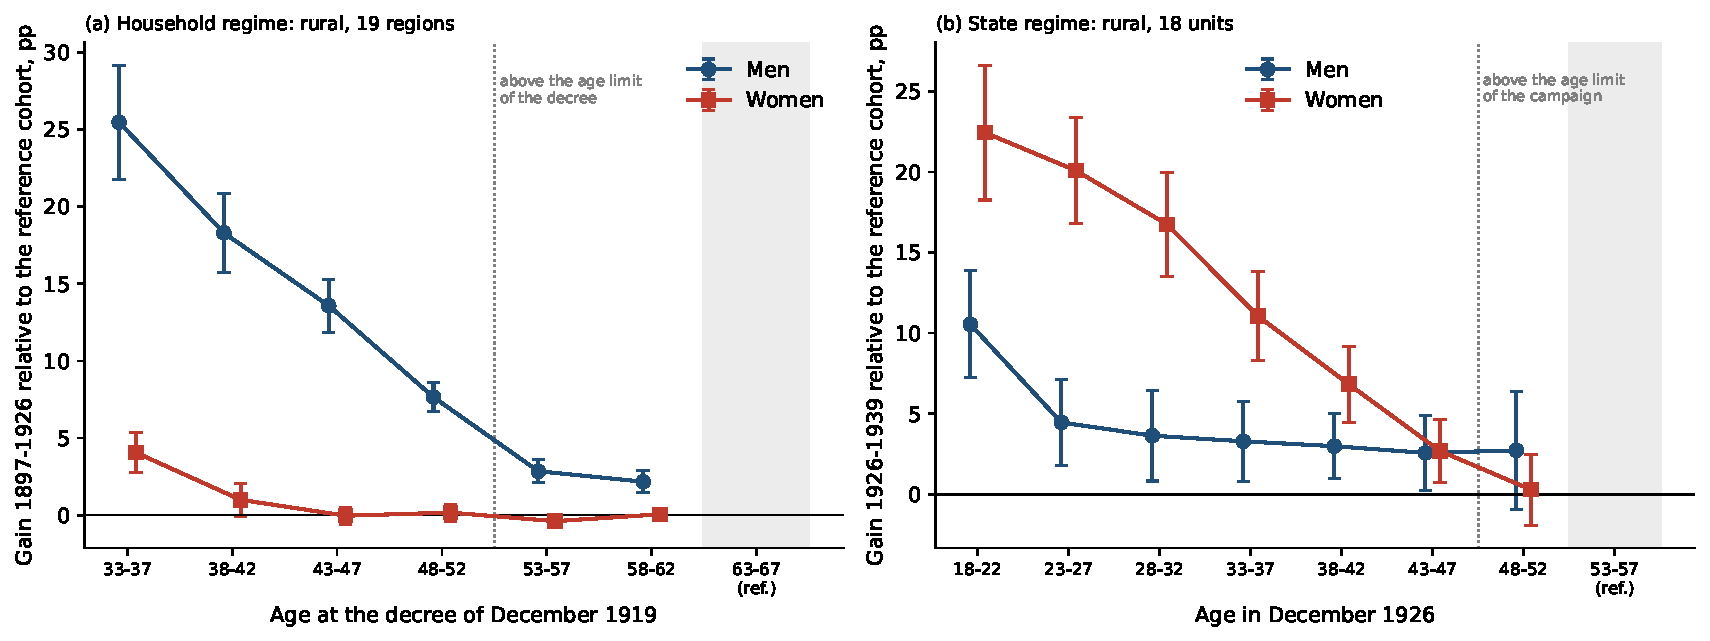
\includegraphics[width=\linewidth]{fig19_event_studies.pdf}
\note{Coefficients relative to the reference cohort with 95 per cent confidence intervals. Panel (a): equation~\eqref{eq:es1}, rural population of \N{w1.regions} regions, reference cohort aged 63 to 67 at the decree. Panel (b): the same specification for 1926 to 1939 in \N{w2.units} units, reference cohort aged 53 to 57 in 1926. The dotted line separates the cohorts above the age limit.}
\end{figure}

\subsection{Robustness}\label{sec:robust1}

The estimates of Table~\ref{tab:es1} are unchanged when unweighted, when the survival ratio is added as a control (its coefficient is \N{w1s.surv} with a standard error of \N{w1s.surv.se}), in the total population, and when the five Muslim regions, where Arabic-script literacy could confound the 1897 baseline, are excluded (Table~\ref{tab:a1}). In the cohorts above the age limit the difference between women and men is \NIA{w1.d.58-62} to \NIA{w1.d.53-57} points, against \NIA{w1.d.43-47} to \NIA{w1.d.33-37} in the cohorts that the decree covered. A wild cluster bootstrap over the \N{w1.regions} regions gives a $p$-value below 0.001 for the pooled triple difference.

The cohorts that gained are also the cohorts that fought in the wars of 1914 to 1921, and their survival ratios are lower for men (\N{w1.surv.M} for the cohort born between 1878 and 1887, rural RSFSR) than for women (\N{w1.surv.F}). Differential mortality by literacy could raise the recorded literacy of survivors without any learning. A bound shows that it cannot account for the result. The excess attrition of men relative to women is \N{w1.excess} per cent of the 1897 male cohort. If every one of these excess losses had been illiterate, male literacy would have risen by \N{w1.bound} points, against an observed gain of \N{w1.gainM}. The cohort above the age limit, whose survival ratio is lower still (\N{w1.surv.placebo}), shows the selection actually realised at higher mortality, \N{w1.gain.placebo} points. The women of the cohorts that gained lost nearly as large a share of their number as the men, and their literacy did not rise, as it would have done had survival depended on literacy to an extent that mattered. Age misreporting is a second concern, since illiterate respondents and women report round ages more often \citep{ahearn2009}. The Whipple index at ages 23 to 62 in 1926 is \N{whipple.M.ill} for illiterate men and \N{whipple.F.ill} for illiterate women against \N{whipple.M.lit} and \N{whipple.F.lit} for the literate. The cohorts of 1926 that are linked to 1939 are centred on the ages ending in 0 and 5, so that heaping in 1926 stays within the cohort. The five-year groups of 1897 and of 1939 begin at those ages. Heaping moves into each group some of the illiterate a year or two younger and out of it some of those just below the next round age, the two movements largely offset each other, and both are present in the comparison cohorts.

\FloatBarrier
\section{The State Regime, 1926 to 1939}\label{sec:wave2}

\subsection{Adult literacy gains}\label{sec:gains2}

Table~\ref{tab:es2} reports the estimates for 1926 to 1939 and Figure~\ref{fig:es}(b) plots them. Relative to the cohort aged 53 to 57 in 1926, which had passed the age limit when the campaign began, rural women aged 18 to 22 gained \NI{w2.f.18-22} points of literacy, women aged 23 to 27 gained \NI{w2.f.23-27}, women aged 28 to 32 gained \NI{w2.f.28-32}, and the three cohorts that follow gained \NI{w2.f.33-37}, \NI{w2.f.38-42} and \NI{w2.f.43-47}. Men aged 18 to 22 gained \NI{w2.m.18-22} points and the men of every older cohort between \N{w2.m.43-47} and \N{w2.m.23-27}. The difference between women and men is \NI{w2.d.18-22} to \NI{w2.d.23-27} points in the three cohorts aged 18 to 32, \NI{w2.d.33-37} and \NI{w2.d.38-42} points in the next two, and nothing at ages 43 to 47. In the cohorts above the age limit it is \N{w2.d.48-52} (standard error \N{w2.d.48-52.se}) and \N{w2.fref} (\N{w2.fref.se}). The pooled triple difference, the cohorts aged 18 to 32 against the cohorts above the age limit and women against men, is \N{w2.ddd} points (\N{w2.ddd.se}), and against the cohorts aged 33 to 47 it is \N{w2.ddd33} (\N{w2.ddd33.se}).

Within cohorts the gender gap fell from \N{w2.gap26.18-22} to \N{w2.gap39.18-22} points for those aged 18 to 22 in 1926, from \N{w2.gap26.23-27} to \N{w2.gap39.23-27} for those aged 23 to 27, and from \N{w2.gap26.28-32} to \N{w2.gap39.28-32} for those aged 28 to 32. For those aged 43 and over it did not move (Figure~\ref{fig:wave2}). The women of these cohorts had grown up under the household regime. Those aged 23 to 32 in 1926 had been 16 to 25 at the decree, \NI{w2.l26.F.28-32} to \NI{w2.l26.F.23-27} per cent of them could read in 1926, and those who learned afterwards did so in their late twenties and their thirties.

\begin{table}[htbp]\centering
\caption{State regime: literacy gain 1926 to 1939 by age in 1926 and sex, rural population}\label{tab:es2}
\begingroup\small
\fitwidth{\begin{tabular}{lccccc}
\toprule
Age in 1926 & Men, $\beta_b$ & Women, $\beta_b+\delta_b$ & Women $-$ men, $\delta_b$ & Cell means, men / women & Gender gap, 1926 to 1939 \\
\midrule
18-22 & 10.6 (1.6) & 22.4 (2.0) & 11.9 (2.1) & 14.5 / 26.6 & 33 to 21 \\
23-27 & 4.5 (1.3) & 20.1 (1.5) & 15.6 (2.2) & 8.0 / 23.8 & 45 to 30 \\
28-32 & 3.6 (1.3) & 16.8 (1.5) & 13.1 (2.2) & 7.7 / 21.0 & 51 to 37 \\
33-37 & 3.3 (1.2) & 11.1 (1.3) & 7.8 (2.1) & 8.2 / 16.1 & 51 to 43 \\
38-42 & 3.0 (0.9) & 6.8 (1.1) & 3.8 (1.9) & 8.0 / 11.9 & 52 to 48 \\
43-47 & 2.6 (1.1) & 2.7 (0.9) & 0.1 (1.5) & 6.4 / 6.5 & 51 to 51 \\
\multicolumn{6}{l}{\textit{Above the age limit of the campaign}} \\
48-52 & 2.7 (1.7) & 0.3 (1.0) & $-$2.4 (2.2) & 7.9 / 5.4 & 41 to 43 \\
53-57 (reference) & 0 & 0.1 (2.0) & 0.1 (2.0) & 4.9 / 5.0 & 36 to 36 \\
\midrule
Triple difference: aged 18-32 $\times$ female, against 48-57 & \multicolumn{5}{c}{14.5 (2.1); leave-one-out 13.3 to 15.8; permutation $p$ $<$0.001; wild bootstrap $p$ 0.001} \\
Aged 33-47 $\times$ female, against 48-57 & \multicolumn{5}{c}{5.3 (1.6)} \\
Aged 18-32 $\times$ female, against 33-47 & \multicolumn{5}{c}{9.2 (1.1)} \\
Linear in age, cohorts aged 18-47 & \multicolumn{5}{c}{men $-$0.31 (0.06) per year; women $-$0.79 (0.06)} \\
Observations; units; $R^2$ & \multicolumn{5}{c}{218; 18; 0.91} \\
\bottomrule
\end{tabular}
}
\note{Equation~\eqref{eq:es1} applied to 1926 and 1939. Percentage points; standard errors clustered by unit in parentheses. Cohorts of 1926 built from validated single years of age and linked to the five-year groups of 1939 twelve years older; rural population of \N{w2.units} units. Unit fixed effects; weights are 1926 cohort populations. The cohort aged 53-57 is the reference. In its row the entry for women is the coefficient on the female indicator, the difference between women and men within the reference cohort. Cell means are weighted by population. The gender gap is male minus female literacy of the same cohort. Robustness in Table~\ref{tab:a2}.}
\endgroup
\end{table}

\subsection{Who was taught}\label{sec:taught}

The share of the illiterate who were taught gives the comparison of the two regimes in its simplest form (Table~\ref{tab:conv} and Figure~\ref{fig:taught}). Of the rural women aged 18 to 32 who were illiterate in 1926, \N{w2c.young.F} per cent could read in 1939, and of the men \N{w2c.young.M} per cent. Under the household regime the shares had been \N{w1c.treated.F} and \N{w1c.treated.M} per cent. In the cohorts above the age limit the shares under the state regime are \N{w2c.placebo.F} and \N{w2c.placebo.M} per cent, so that relative to them the state regime taught \NI{w2c.dd.women} per cent of the illiterate women (standard error \N{w2c.dd.women.se}) and \NI{w2c.dd.men} per cent of the illiterate men (\N{w2c.dd.men.se}).

\begin{table}[htbp]\centering
\caption{The illiterate who became literate, by regime, cohort and sex, rural population}\label{tab:conv}
\begingroup\small
\fitwidth{\begin{tabular}{lccccccc}
\toprule
 & \multicolumn{3}{c}{Men} & \multicolumn{3}{c}{Women} & Women $-$ men, \\
\cmidrule(lr){2-4}\cmidrule(lr){5-7}
Cohort & Literate before & Literate after & Taught & Literate before & Literate after & Taught & taught \\
\midrule
\multicolumn{8}{l}{\textit{A. Household regime, 1897 to 1926, by age at the decree of 1919}} \\
33-37 & 44 & 66 & 40.0 (3.5) & 15 & 17 & 2.8 (1.0) & $-$37.2 (3.0) \\
38-42 & 43 & 58 & 26.9 (2.5) & 14 & 13 & $-$0.8 (1.0) & $-$27.8 (2.1) \\
43-47 & 38 & 49 & 17.4 (1.8) & 11 & 10 & $-$2.0 (0.7) & $-$19.3 (1.5) \\
48-52 & 38 & 42 & 7.7 (1.3) & 9 & 8 & $-$1.7 (0.7) & $-$9.4 (0.7) \\
53-57 & 36 & 36 & 0.0 (1.2) & 8 & 6 & $-$2.3 (0.5) & $-$2.3 (0.9) \\
58-62 & 33 & 32 & $-$1.0 (1.2) & 7 & 5 & $-$1.8 (0.5) & $-$0.8 (0.8) \\
63-67 & 29 & 26 & $-$4.0 (1.0) & 6 & 4 & $-$1.8 (0.5) & 2.2 (0.7) \\
Aged 33-47 against 53-67 & & & 31.3 (3.0) & & & 2.2 (0.5) & $-$29.1 (2.8) \\
\midrule
\multicolumn{8}{l}{\textit{B. State regime, 1926 to 1939, by age in 1926}} \\
18-22 & 80 & 94 & 71.6 (1.3) & 47 & 74 & 50.2 (2.3) & $-$21.4 (2.2) \\
23-27 & 85 & 93 & 52.6 (2.7) & 39 & 63 & 39.2 (2.6) & $-$13.4 (2.5) \\
28-32 & 82 & 89 & 42.0 (2.3) & 31 & 52 & 30.5 (2.4) & $-$11.6 (2.0) \\
33-37 & 76 & 84 & 33.4 (2.6) & 25 & 41 & 21.4 (2.0) & $-$12.0 (2.7) \\
38-42 & 68 & 76 & 25.3 (2.2) & 17 & 29 & 14.3 (1.9) & $-$11.0 (3.2) \\
43-47 & 63 & 69 & 17.2 (2.0) & 12 & 18 & 7.4 (1.8) & $-$9.8 (2.8) \\
48-52 & 49 & 56 & 15.3 (3.1) & 9 & 14 & 5.9 (2.0) & $-$9.4 (3.7) \\
53-57 & 43 & 48 & 8.7 (1.6) & 7 & 12 & 5.4 (2.1) & $-$3.3 (2.5) \\
Aged 18-32 against 48-57 & & & 49.6 (2.5) & & & 37.2 (2.1) & $-$12.5 (2.7) \\
\bottomrule
\end{tabular}
}
\note{Literate before and after are the literacy rates of the cohort at the earlier and the later census, in per cent. Taught is the change in literacy divided by the share illiterate at the earlier census, equation~\eqref{eq:taught}, in per cent, weighted by the number of illiterate at the earlier census, with standard errors clustered by region (panel A) or unit (panel B) in parentheses. The last row of each panel is the difference between the cohorts the regime could reach and the cohorts above the age limit, with region or unit fixed effects. Samples as in Tables~\ref{tab:es1} and~\ref{tab:es2}.}
\endgroup
\end{table}

Two conclusions follow. The first is that the state regime did not favour women over men. An illiterate man was still more likely to be taught than an illiterate woman, by \NIA{w2c.dif.43-47} to \NIA{w2c.dif.18-22} points at every age below the limit. Relative to the cohorts above the limit the difference between women and men in the share taught is \N{w2c.dd.dif} points (\N{w2c.dd.dif.se}), and \N{w2c.ddd} (\N{w2c.ddd.se}) when each cohort is given its own effect. The larger gains of women in percentage points come from the composition of the illiterate. Women were \N{w2c.share.ill.F} per cent of the illiterate of these cohorts in 1926 and \N{w2c.share.new.F} per cent of those who learned. The second is that the difference between the regimes lies in the appearance of women among the taught. The ratio of the female share to the male share rose from \N{w1c.ratio} to \N{w2c.ratio}.

The two regimes can also be compared on cohorts that were young adults when each period began. Under the household regime the cohorts aged 38 to 47 at the decree were 15 to 24 years old in 1897. Of their illiterate men \NI{w1c.M.38-42} and \NI{w1c.M.43-47} per cent were taught in the thirty years that followed, and of their illiterate women none. Under the state regime the cohorts aged 18 to 32 in 1926 were of similar ages at the start of the period. Of their illiterate men \N{w2c.young.M} per cent were taught in twelve years and of their illiterate women \N{w2c.young.F}. The state regime therefore raised the rate at which illiterate men were taught as well, and it brought women from nothing to two thirds of that rate.

Equation~\eqref{eq:mix} gives the two shares a simple reading. If the household component of women is zero, the share of illiterate women who were taught measures the reach of the state among women, \N{mix.e}. If the reach were the same among men, their share would exceed it by $(1-e)H_m$, where $H_m$ is the share of men who would have learned without the campaign, at home, in the army or at work. With the share of men of the same ages taught under the household regime, \N{mix.h.adult}, in the place of $H_m$, the predicted share of men is \N{mix.pred.adult}, and the observed share is \N{mix.obs}. The routes that had been open to men before the campaign thus account for \N{mix.gap.pred} of the \N{mix.gap.obs} points by which the share of men exceeds that of women. The remainder indicates that the instruments of the state reached men somewhat more than women, as condition~\eqref{eq:state} allows and as the separate instruction of men about to be conscripted would produce, or that the earlier routes had widened by the 1930s. The lengths of the two periods differ, and the division should not be pressed.

Hypothesis H2 concerns age. Under the household regime the share of illiterate men who were taught fell from \NI{w1c.M.33-37} per cent at ages 33 to 37 to nothing above the age limit, and the share of women was nil at every age. Under the state regime the shares of both sexes fall with age, by \NA{w2c.age.m} points per year for men and \NA{w2c.age.f} for women, and reach the level of the cohorts above the age limit between the ages of 43 and 52. The excess of men over women, as a share of the men whom a reach equal to that of women would leave out, is \N{mixh.18-22} per cent at ages 18 to 22, \N{mixh.23-27} at 23 to 27, \N{mixh.28-32} at 28 to 32 and \N{mixh.43-47} at 43 to 47. It declines with age as the hypothesis requires and as the share of men taught under the household regime had done, which was \NI{w1c.M.38-42} per cent among those aged 15 to 19 at the start of that period, \NI{w1c.M.48-52} among those aged 25 to 29 and nothing above 30. The decline of the share of women, which is the state's reach, is gradual, and the age limit is not visible in it as a discontinuity. A cost of teaching that rises with age produces this, and a rule applied by age alone would not.

\FloatBarrier
\subsection{Robustness}\label{sec:robust2}

The sample of the state regime has \N{w2.units} units, and several checks speak to the concern that so few units drive the result. The leave-one-unit-out estimates of the pooled triple difference range from \N{w2.loo.min} to \N{w2.loo.max} (Figure~\ref{fig:inference}). The distribution of the coefficient under random reassignment of the sexes within unit and cohort has 95 per cent of its mass between \N{w2.perm.lo} and \N{w2.perm.hi}, against an observed \N{w2.ddd}. A restricted wild cluster bootstrap over the shared 1939 source territories gives a Monte Carlo $p$-value of \N{w2.wild}. And the analysis replicates at the level of the \N{ray.units} Gosplan regions, which cover the entire RSFSR, using Table XV for 1926 and the 1939 oblasts aggregated to regions (Figure~\ref{fig:rayons}). At that level the pooled triple difference is \N{ray.ddd} (\N{ray.ddd.se}), or \N{ray.ddd.exact} (\N{ray.ddd.exact.se}) in the \N{ray.units.exact} regions whose 1926 and 1939 borders coincide, and the gender gap within cohorts falls from \N{ray.gap26.20-24} to \N{ray.gap39.20-24} points for those aged 20 to 24 in 1926 and from \N{ray.gap26.25-29} to \N{ray.gap39.25-29} for those aged 25 to 29. In the rural RSFSR as a whole \N{ray.c.young.F} per cent of the women aged 20 to 34 who were illiterate in 1926 could read in 1939, and \N{ray.c.young.M} per cent of the men, and women were \N{ray.c.share.ill.F} per cent of the illiterate. The shares are lower than in the sample of units, in which the cohorts are two years younger and exactly matched, and their ratio, \N{ray.c.ratio}, is close to the \N{w2c.ratio} of the sample.

The borders of units changed between the censuses, and the sizes of cohorts changed with them. Adding the survival ratio as a control leaves the triple difference at \N{w2r.surv.ddd} (\N{w2r.surv.ddd.se}). Restricting the sample to the cells whose cohorts changed in size by no more than mortality and ordinary migration would imply, with survival ratios between 0.6 and 1.15, gives \N{w2r.sr.ddd} (\N{w2r.sr.ddd.se}) on \N{w2r.sr.nunits} units. Excluding the Ural \emph{okrugi} gives \N{w2r.ural.ddd}, excluding the Tatar and Bashkir republics, where Latinisation could have reduced the recorded Arabic-script literacy, gives \N{w2r.mus.ddd}, excluding the six low-quality units \N{w2r.low.ddd}, the total population \N{w2r.total.ddd} and the cells validated at the first test alone \N{w2r.t1.ddd} (Table~\ref{tab:a2}). The triple difference in the share taught, with cohort effects, is between \N{w2c.sr.ddd} and \N{w2c.unw.ddd} across the same variations, and the share of illiterate women who were taught between \N{w2c.unw.young.F} and \N{w2c.total.young.F} per cent.

The gains could be an artefact of an inflated 1939 count, since the campaign was a political target and the census that followed the suppressed census of 1937 was taken under pressure. Four features of the results speak against this reading. The definition of literacy did not change between the censuses. An enumerator who recorded the illiterate as literate at every age would not have produced a share of the illiterate recorded as literate that falls from \NI{w2c.F.18-22} per cent of women aged 18 to 22 to \NI{w2c.F.53-57} per cent of women aged 53 to 57, and the oldest cohorts bound what a uniform inflation could have added. The overcount of the population, which \citet{zhiromskaya2001} puts at 1.7 per cent, would raise a literacy rate by less than two points even if every person added had been entered as literate.

The census of 1959 is an additional consistency check, not a bound on the error of the census of 1939. Subsequent learning, loss of skills, selection and territorial changes can offset a reporting error. High literacy in 1959 therefore supports persistence among surviving cohorts without identifying when all of them learned.

The pooled population ratio of the original unit sample cannot bound mortality or out-migration because the territories differ, and some 1939 populations are reused. Accounting bounds require common territories and explicit assumptions about gross inflows. Sensitivity to these assumptions is reported separately.

\begin{table}[htbp]\centering
\caption{The cohorts of 1926 in the censuses of 1939 and 1959, RSFSR}\label{tab:c59}
\begingroup\small
\begin{tabular}{lcccccc}
\toprule
 & \multicolumn{3}{c}{Men} & \multicolumn{3}{c}{Women} \\
\cmidrule(lr){2-4}\cmidrule(lr){5-7}
Age in 1926 & 1926 & 1939 & 1959 & 1926 & 1939 & 1959 \\
\midrule
\multicolumn{7}{l}{\textit{A. Rural population}} \\
20-24 & 83.0 & 92.9 & 94.3 & 50.5 & 69.8 & 70.7 \\
25-29 & 82.2 & 90.9 & 91.5 & 39.8 & 59.4 & 57.8 \\
30-34 & 79.5 & 87.3 & 87.8 & 33.8 & 48.1 & 46.5 \\
20-34 & 81.9 & 90.9 & 91.7 & 42.6 & 60.7 & 60.1 \\
Share of the illiterate of 1926 literate, 20-34 & & 50 & 54 & & 32 & 31 \\
\midrule
\multicolumn{7}{l}{\textit{B. Whole population}} \\
20-24 & 86.0 & 94.8 & 95.8 & 58.0 & 77.3 & 76.5 \\
25-29 & 85.2 & 93.2 & 93.7 & 49.1 & 68.8 & 66.0 \\
30-34 & 83.1 & 90.5 & 90.6 & 43.5 & 58.9 & 56.1 \\
20-34 & 85.0 & 93.2 & 93.8 & 51.2 & 69.7 & 67.6 \\
Share of the illiterate of 1926 literate, 20-34 & & 55 & 59 & & 38 & 34 \\
\bottomrule
\end{tabular}

\note{Literate persons per hundred. The 1926 figures are those of Table XV of Volume 9 for the \N{c3.regions} regions that formed the RSFSR of 1939; the 1939 and 1959 figures are sums over the RSFSR. A five-year group of 1926 is twelve years older in January 1939 and thirty-two years older in January 1959, and is matched in each census to three fifths of one five-year group and two fifths of the next. In 1959 the literate are those with any schooling and those without schooling who can read. The last row of each panel gives the change since 1926 as a share of those illiterate in 1926.}
\endgroup
\end{table}

\begin{table}[htbp]\centering
\caption{The five-year groups of 1926 in the census of 1939, RSFSR}\label{tab:c4}
\begingroup\small
\fitwidth{\begin{tabular}{lcccccccccccc}
\toprule
 & \multicolumn{6}{c}{Rural population} & \multicolumn{6}{c}{Whole population} \\
\cmidrule(lr){2-7}\cmidrule(lr){8-13}
 & \multicolumn{3}{c}{Women} & \multicolumn{3}{c}{Men} & \multicolumn{3}{c}{Women} & \multicolumn{3}{c}{Men} \\
\cmidrule(lr){2-4}\cmidrule(lr){5-7}\cmidrule(lr){8-10}\cmidrule(lr){11-13}
Age in 1926 & 1926 & 1939 & Taught & 1926 & 1939 & Taught & 1926 & 1939 & Taught & 1926 & 1939 & Taught \\
\midrule
20-24 & 50.5 & 69.8 & 39 & 83.0 & 92.9 & 58 & 58.0 & 77.3 & 46 & 86.0 & 94.8 & 63 \\
25-29 & 39.8 & 59.4 & 33 & 82.2 & 90.9 & 49 & 49.1 & 68.8 & 39 & 85.2 & 93.2 & 54 \\
30-34 & 33.8 & 48.1 & 22 & 79.5 & 87.3 & 38 & 43.5 & 58.9 & 27 & 83.1 & 90.5 & 43 \\
35-39 & 26.2 & 36.4 & 14 & 75.1 & 82.3 & 29 & 35.1 & 47.5 & 19 & 79.1 & 86.4 & 35 \\
40-44 & 18.1 & 25.0 & 8 & 68.7 & 75.5 & 22 & 26.2 & 35.8 & 13 & 73.4 & 80.7 & 27 \\
45-49 & 13.7 & 17.7 & 5 & 60.9 & 65.3 & 11 & 21.2 & 26.8 & 7 & 66.1 & 71.6 & 16 \\
50-54 & 10.2 & 13.4 & 3 & 52.5 & 56.3 & 8 & 17.0 & 21.7 & 6 & 58.2 & 62.5 & 10 \\
\bottomrule
\end{tabular}
}
\note{Literate persons per hundred in 1926 (Table XV of Volume 9, the \N{c3.regions} regions that formed the RSFSR of 1939) and in 1939 (sums over the RSFSR, each five-year group of 1926 being matched to three fifths of one five-year group of 1939 and two fifths of the next). Taught is the change as a share of those illiterate in 1926, in per cent.}
\endgroup
\end{table}

\FloatBarrier

\section{Regions and the Move to the Towns}\label{app:why}

Figure~\ref{fig:why} shows the regional test of Section~\ref{sec:why}. Each point is one of the \N{mech.n} regions that made up the RSFSR of 1939, and the horizontal axis is the change in the share of the cohort aged 20 to 34 in 1926 that lived in towns, a measure of how far the opportunities of the new economy reached the region and of how many of its young people left the village.

\begin{figure}[htbp]\centering
\caption{The share of illiterate women who learned and the move of their cohort to the towns, by region}\label{fig:why}
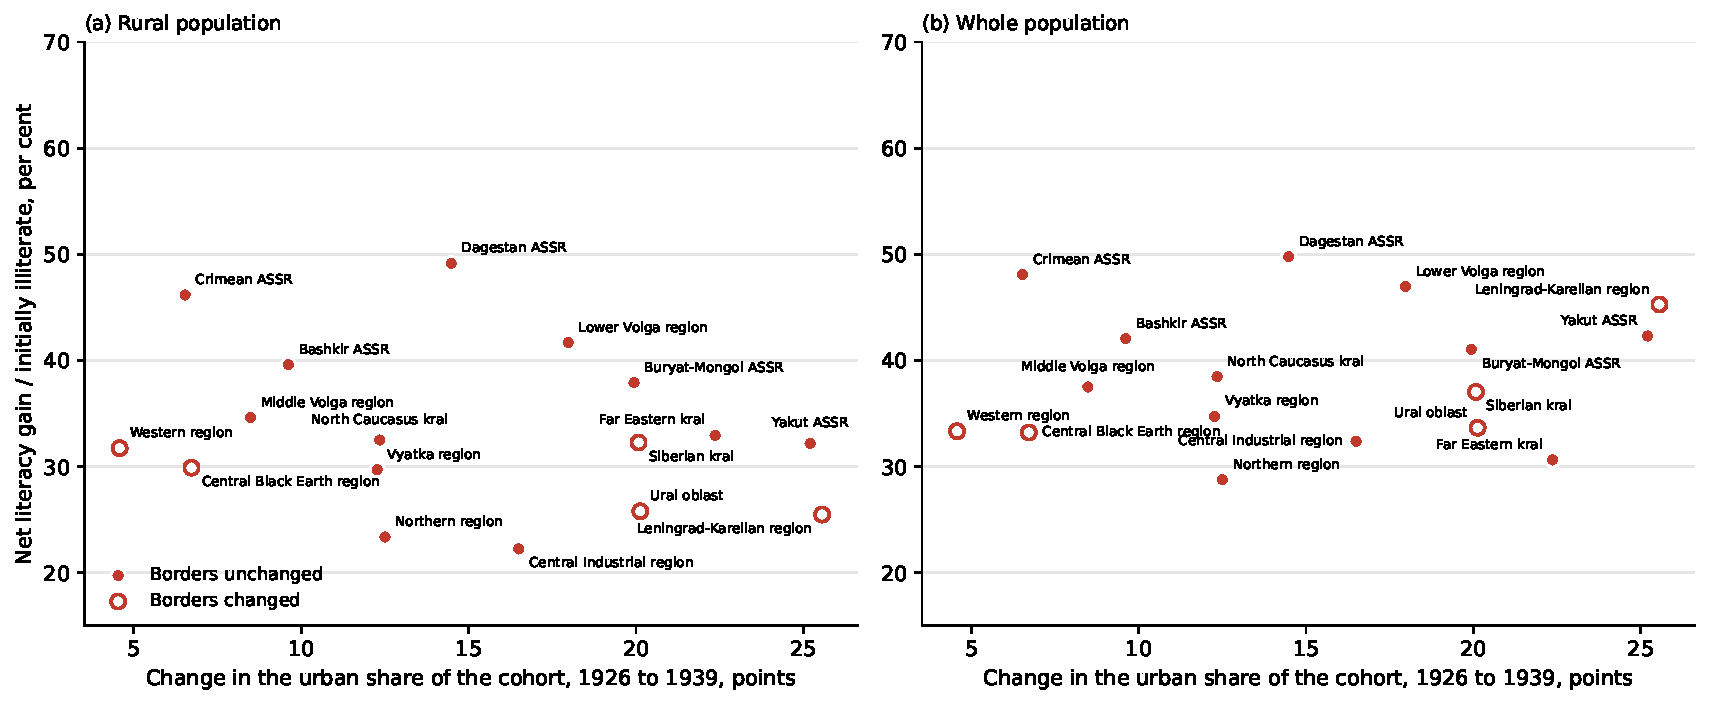
\includegraphics[width=\linewidth]{fig29_why_regions.pdf}
\note{Cohort aged 20 to 34 in 1926, women. The vertical axis is the change in literacy between 1926 and 1939 divided by the share illiterate in 1926. The horizontal axis is the change in the urban share of the same cohort, computed as one minus the ratio of its rural to its total number in each census. Filled points mark the regions whose borders did not change. Panel (a): rural population. Panel (b): whole population.}
\end{figure}

\FloatBarrier
\section{Additional Tables and Figures}\label{app:tables}

\begin{figure}[htbp]\centering
\caption{Literacy by year of birth as recorded by four censuses, by sex and population}\label{fig:mainall}
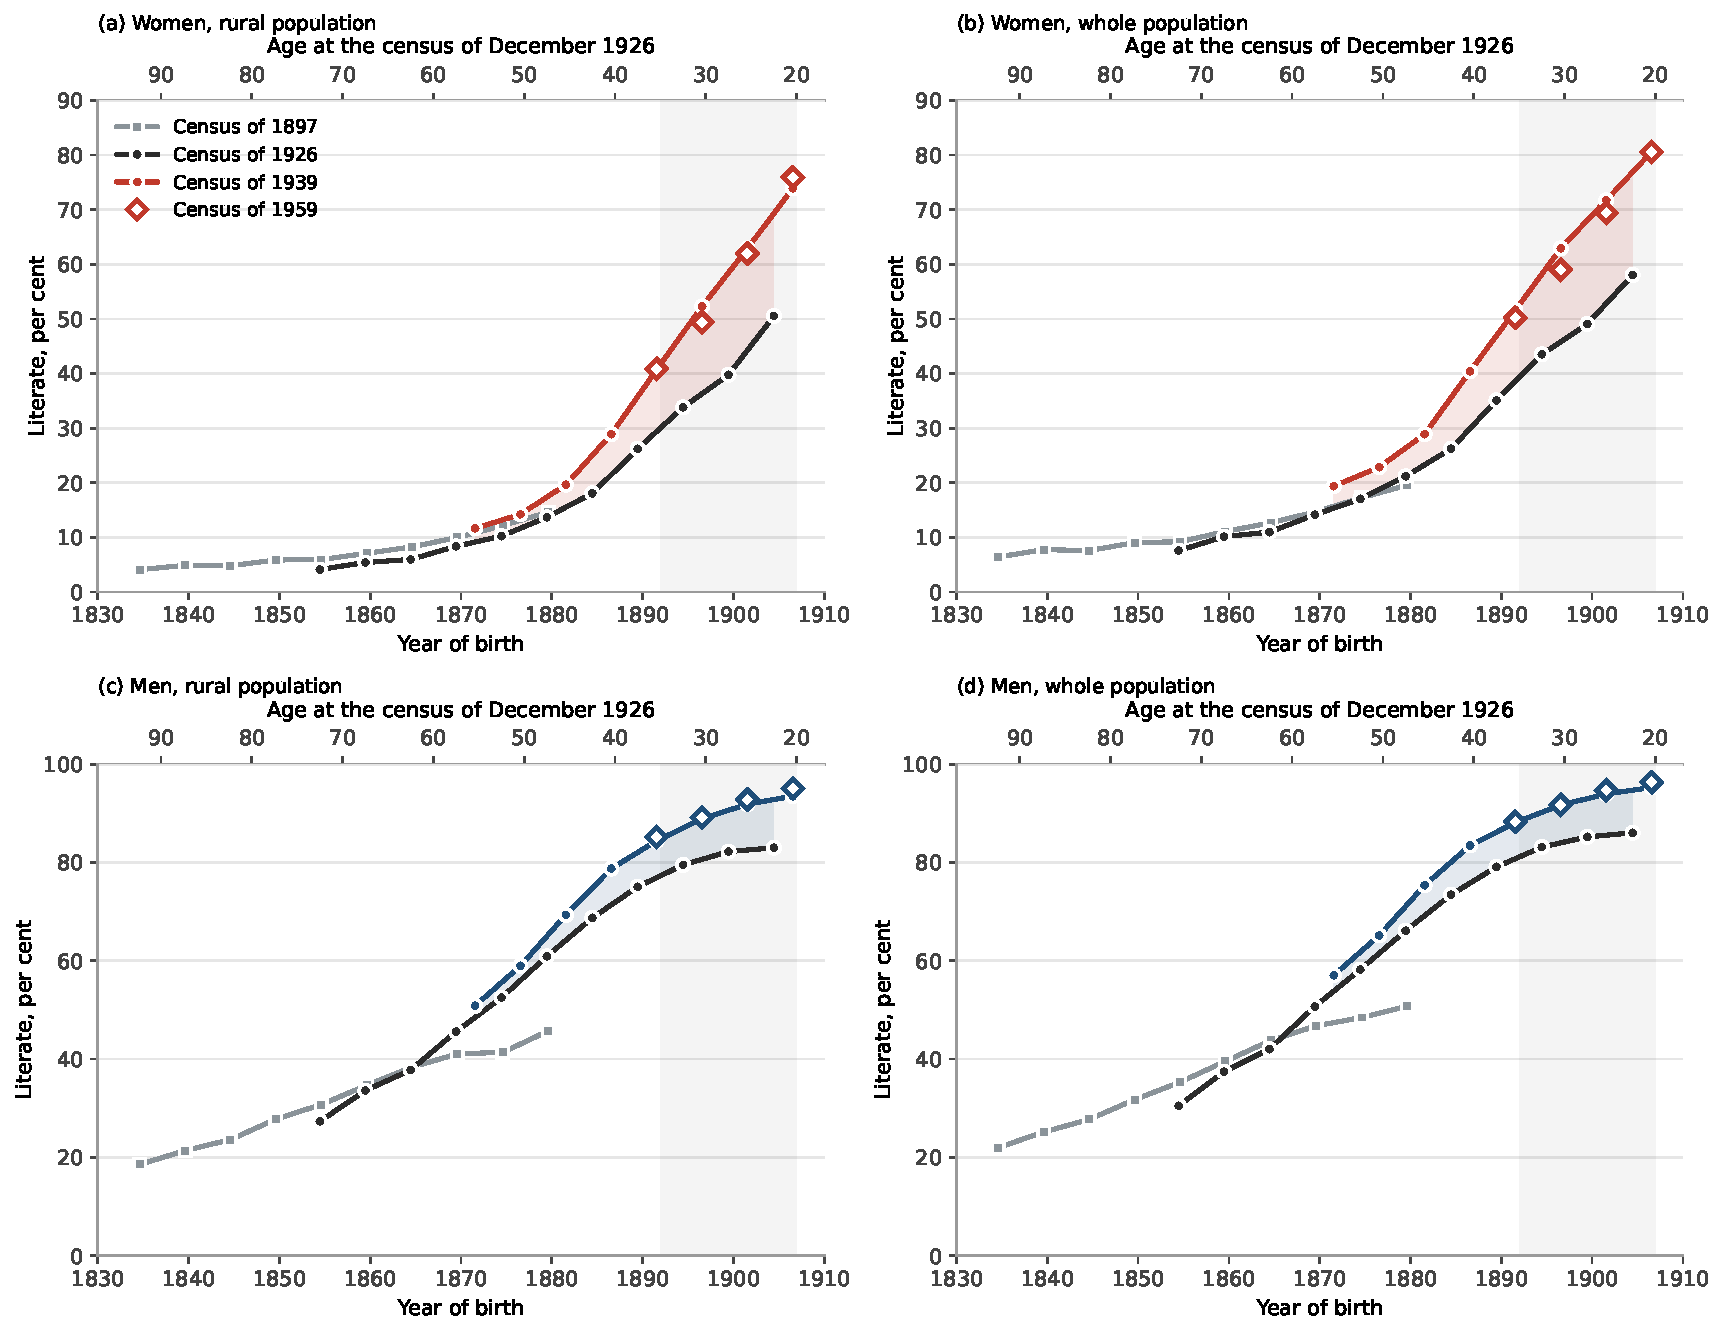
\includegraphics[width=\linewidth]{fig26_cohorts_all.pdf}
\note{As Figure~\ref{fig:main}, which is repeated in panel (a), for the whole population of the RSFSR and for men. Each point is a five-year age group of the census named, placed at its mean year of birth; the upper axis gives the age of the cohort in December 1926 and the grey band marks the cohort aged 20 to 34. The censuses of 1939 and 1959 are drawn in red for women and in blue for men. Among men the census of 1926 lies above that of 1897 for the cohorts born after 1865, who learned as adults before the campaign.}
\end{figure}

\begin{table}[htbp]\centering
\caption{Household regime: robustness of the estimates by cohort}\label{tab:a1}
\begingroup\small
\fitwidth{\begin{tabular}{lccccc}
\toprule
Specification & Men 33-42 & Men 43-52 & $\times$ female 33-42 & $\times$ female 43-52 & $n$ \\
\midrule
Baseline (rural, weighted; ten-year cohorts, reference 53-62) & 19.2 (1.7) & 8.0 (0.7) & $-$16.5 (1.9) & $-$7.8 (0.7) & 113 \\
Unweighted & 18.5 (1.6) & 7.5 (0.7) & $-$15.8 (1.5) & $-$7.3 (0.7) & 113 \\
With survival ratio & 19.5 (1.9) & 8.4 (1.0) & $-$16.7 (2.0) & $-$8.0 (0.8) & 113 \\
Excluding Muslim regions & 20.3 (1.9) & 8.5 (0.7) & $-$17.4 (2.1) & $-$8.3 (0.8) & 84 \\
Survival ratio in $[0.4, 0.8]$ & 19.0 (1.8) & 8.1 (0.9) & $-$16.2 (2.1) & $-$8.0 (1.0) & 90 \\
Total population & 20.0 (1.7) & 8.1 (0.6) & $-$15.5 (2.0) & $-$7.3 (0.7) & 113 \\
Urban population & 3.7 (2.0) & 5.9 (0.9) & $-$6.6 (0.8) & $-$5.5 (0.9) & 114 \\
\midrule
Five-year bins (Table~\ref{tab:es1}), $\delta_b$ for 33-37 / 38-42 / 43-47 & \multicolumn{5}{c}{$-$21.4 (2.0) / $-$17.3 (1.4) / $-$13.6 (0.9)} \\
Five-year bins, unweighted & \multicolumn{5}{c}{$-$20.7 (1.7) / $-$16.8 (1.3) / $-$12.8 (1.2)} \\
Five-year bins, with survival ratio & \multicolumn{5}{c}{$-$21.5 (2.0) / $-$17.6 (1.3) / $-$14.0 (0.9)} \\
Five-year bins, total population & \multicolumn{5}{c}{$-$20.1 (2.2) / $-$16.4 (1.6) / $-$12.4 (0.9)} \\
Triple difference without the cohort aged 33-37 & \multicolumn{5}{c}{$-$13.9 (1.2); men aged 38-47 against 53-67: 14.5 (1.1)} \\
\bottomrule
\end{tabular}
}
\note{Percentage points; standard errors clustered by region in parentheses. Upper panel: ten-year cohorts aged 33-42 and 43-52 at the decree against the cohort aged 53-62; region fixed effects. Lower panel: equation~\eqref{eq:es1} with five-year bins.}
\endgroup
\end{table}

\begin{table}[htbp]\centering
\caption{State regime: robustness of the difference between women and men by cohort}\label{tab:a2}
\begingroup\footnotesize
\fitwidth{\begin{tabular}{lccccccccc}
\toprule
 & \multicolumn{7}{c}{Female excess gain $\delta_b$ by age in 1926} & Triple & Cells; \\
\cmidrule(lr){2-8}
Specification & 18-22 & 23-27 & 28-32 & 33-37 & 38-42 & 43-47 & 48-52 & difference & units \\
\midrule
Baseline & 11.9 (2.1) & 15.6 (2.2) & 13.1 (2.2) & 7.8 (2.1) & 3.8 (1.9) & 0.1 (1.5) & $-$2.4 (2.2) & 14.5 (2.1) & 218; 18 \\
Including flagged units & 10.6 (2.3) & 14.0 (2.6) & 11.7 (2.4) & 6.5 (2.3) & 3.1 (1.9) & $-$0.4 (1.5) & $-$2.4 (1.9) & 13.1 (2.4) & 250; 20 \\
With survival ratio & 11.4 (2.2) & 15.0 (2.3) & 12.7 (2.3) & 7.6 (2.2) & 3.6 (1.9) & 1.1 (1.4) & $-$2.4 (2.1) & 13.6 (2.1) & 218; 18 \\
Survival ratio in $[0.6, 1.15]$ & 8.0 (2.4) & 11.4 (2.2) & 8.8 (2.1) & 3.6 (1.8) & $-$0.3 (1.3) & $-$2.2 (2.0) & $-$2.0 (1.5) & 10.4 (1.9) & 124; 12 \\
Unweighted & 11.8 (1.9) & 14.9 (1.9) & 12.0 (1.9) & 6.0 (1.8) & 1.3 (1.6) & $-$1.5 (1.4) & $-$3.0 (2.2) & 14.2 (2.1) & 218; 18 \\
Russian units only & 13.4 (1.8) & 17.1 (2.1) & 14.5 (2.4) & 9.8 (2.5) & 5.6 (2.4) & 1.6 (1.4) & $-$0.3 (1.7) & 14.9 (2.0) & 138; 12 \\
Excluding Ural okrugi & 11.9 (2.2) & 15.7 (2.3) & 13.2 (2.3) & 8.0 (2.3) & 4.1 (2.0) & 0.3 (1.6) & $-$2.5 (2.3) & 14.6 (2.2) & 178; 15 \\
Excluding Tatar and Bashkir republics & 14.1 (1.6) & 17.5 (1.8) & 14.8 (2.1) & 9.6 (2.0) & 4.7 (2.0) & 1.1 (1.2) & $-$1.9 (2.2) & 16.3 (1.9) & 194; 16 \\
Excluding low-quality units & 12.7 (2.1) & 16.5 (2.2) & 14.0 (2.3) & 8.0 (2.2) & 4.0 (1.9) & 0.3 (1.6) & $-$1.4 (2.5) & 14.8 (2.5) & 192; 15 \\
Cells validated by the first rule only & 12.1 (2.1) & 15.6 (2.2) & 13.1 (2.2) & 7.8 (2.1) & 3.8 (1.9) & 0.1 (1.5) & $-$1.5 (2.2) & 14.1 (2.3) & 214; 17 \\
Units with all eight cohorts & 13.8 (3.4) & 17.9 (3.0) & 15.4 (3.2) & 8.9 (2.9) & 5.4 (2.2) & 2.0 (0.9) & 0.3 (0.4) & 15.4 (3.2) & 112; 7 \\
Total population & 12.1 (1.3) & 15.3 (1.3) & 12.1 (2.4) & 7.5 (1.3) & 5.1 (1.5) & 0.8 (1.0) & $-$0.1 (0.4) & 13.3 (1.4) & 352; 25 \\
\bottomrule
\end{tabular}
}
\note{Coefficients $\delta_b$ of equation~\eqref{eq:es1} applied to 1926 and 1939, relative to the cohort aged 53-57, and the pooled triple difference of the cohorts aged 18-32 against those aged 48-57. Unit fixed effects; standard errors clustered by unit.}
\endgroup
\end{table}

\begin{figure}[htbp]\centering
\caption{The state regime: gains of the same cohorts and the gender gap within cohorts}\label{fig:wave2}
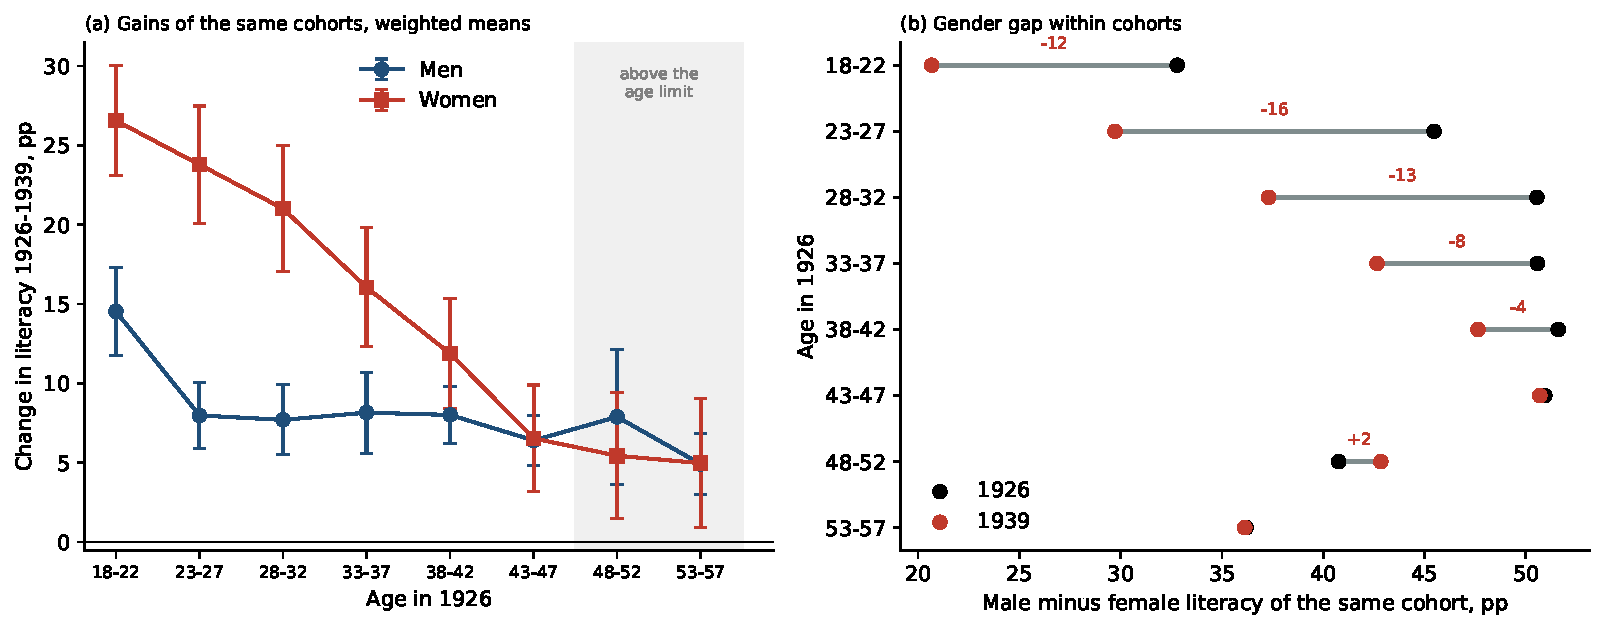
\includegraphics[width=\linewidth]{fig04_wave2_linked_cohorts.pdf}
\note{Panel (a): population-weighted mean gains with 95 per cent confidence intervals, rural population of \N{w2.units} units. Panel (b): male minus female literacy of the same cohort in 1926 and in 1939.}
\end{figure}

\begin{figure}[htbp]\centering
\caption{Inference for the triple difference of the state regime}\label{fig:inference}
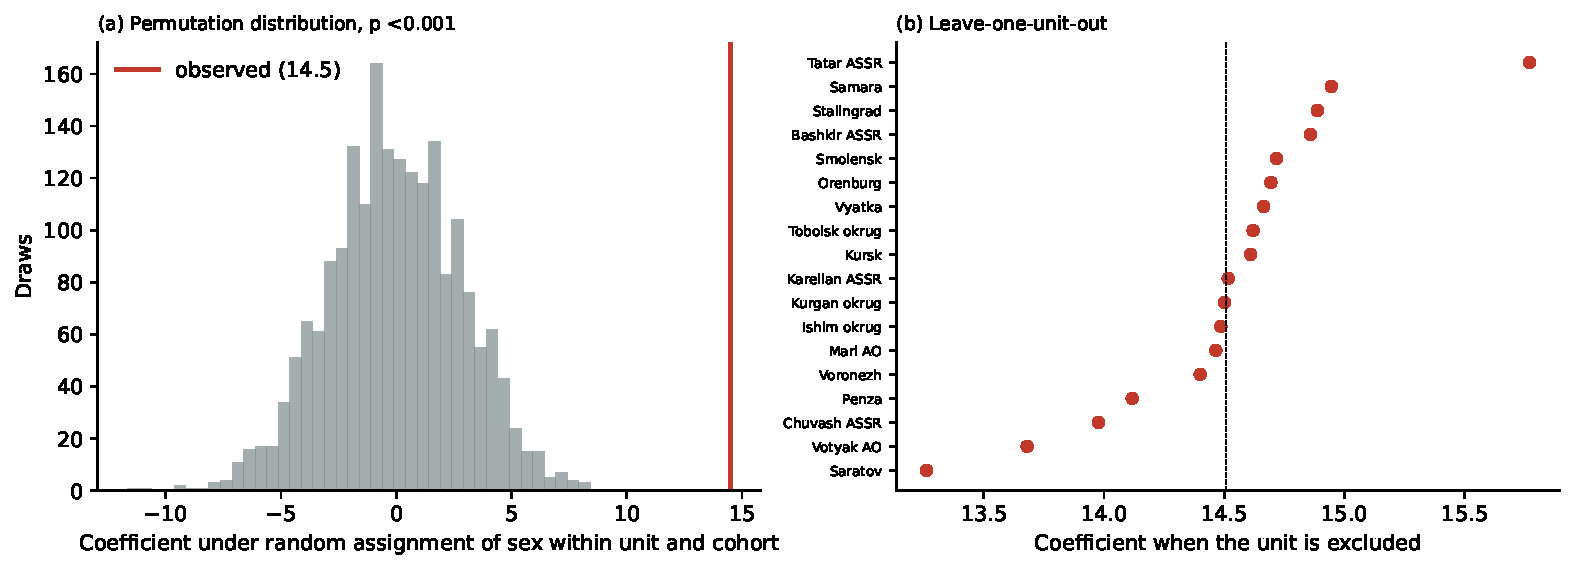
\includegraphics[width=\linewidth]{fig13_inference.pdf}
\note{Panel (a): distribution of the pooled triple-difference coefficient under 2,000 random reassignments of the sexes within unit and cohort. Panel (b): the coefficient when each unit in turn is excluded.}
\end{figure}

\begin{figure}[htbp]\centering
\caption{Replication of the state regime at the level of Gosplan regions}\label{fig:rayons}
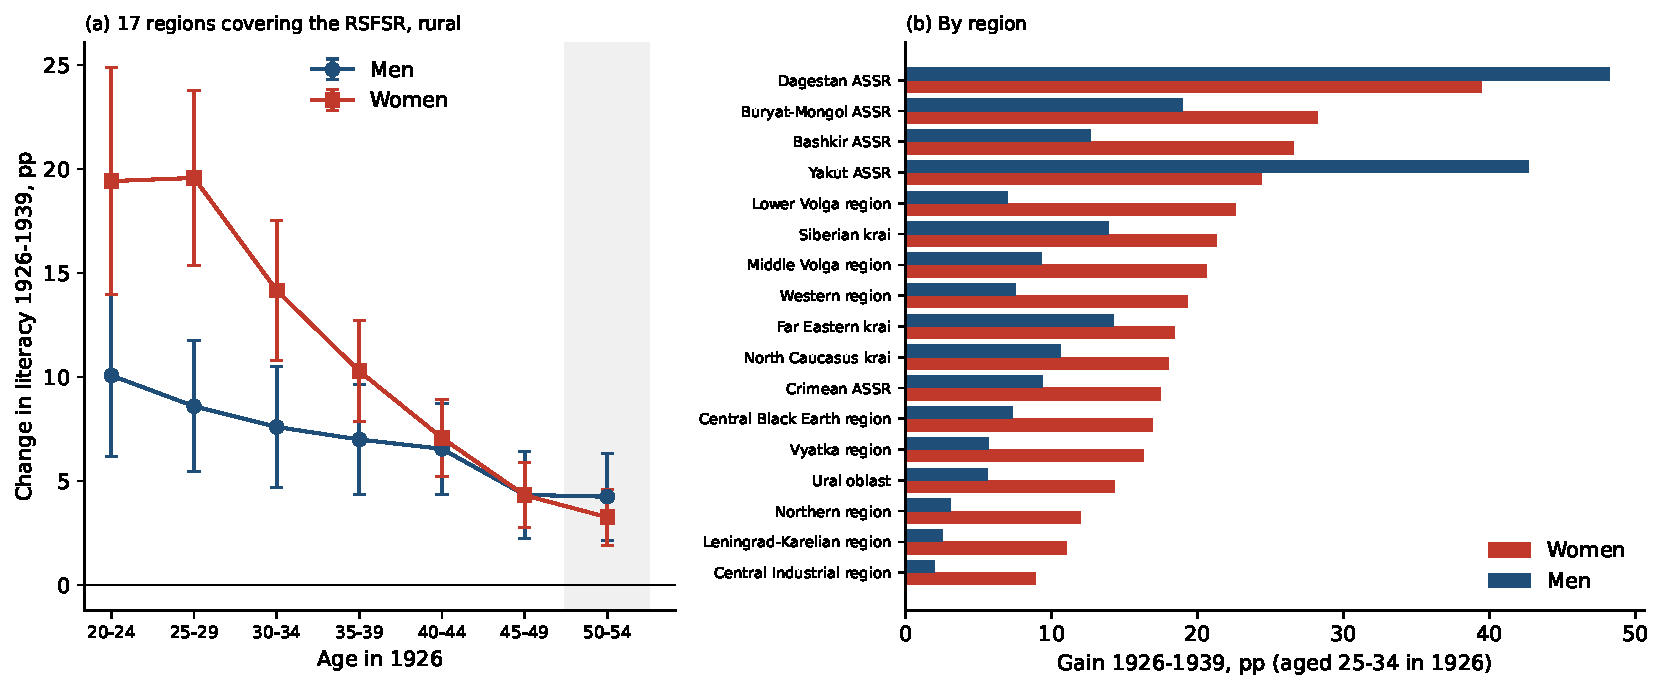
\includegraphics[width=\linewidth]{fig16_wave2_rayons.pdf}
\note{1926 from Vol.\ 9, Table XV; 1939 oblasts aggregated to the \N{ray.units} regions. Because the five-year bands of 1926 shift by twelve years, each band is matched to a mixture of the two overlapping bands of 1939 in the proportion three to two. The shaded cohort was above the age limit.}
\end{figure}

\begin{figure}[htbp]\centering
\caption{Gains under the state regime by unit and cohort}\label{fig:dose}
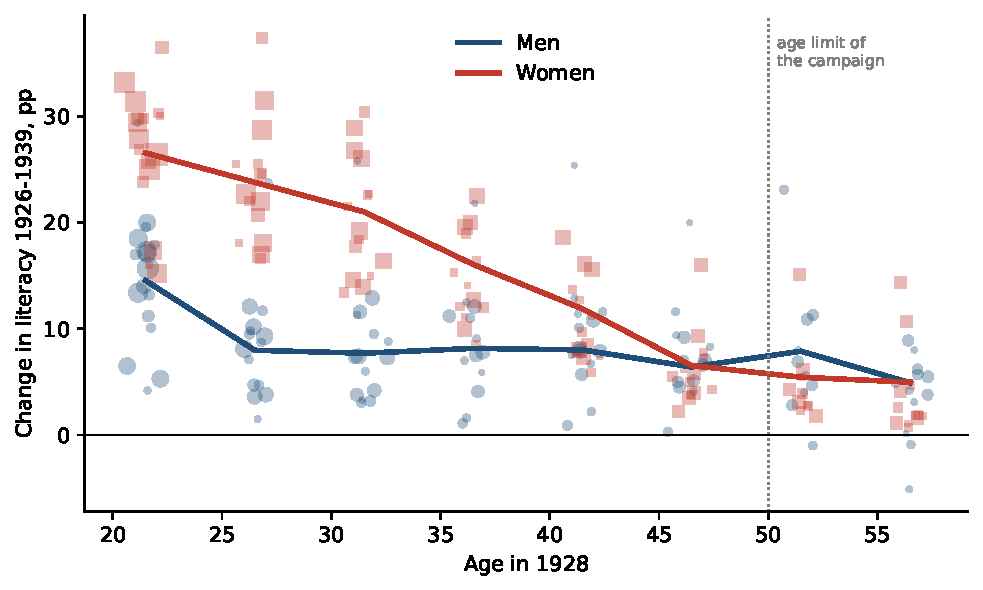
\includegraphics[width=0.8\linewidth]{fig05_dose_response_wave2.pdf}
\note{Cells by unit and cohort, rural population, sized by 1926 population; lines join population-weighted means.}
\end{figure}

\clearpage
\section{New regional follow-up and institutional evidence}\label{app:newdata}
% Generated by scripts/write_supplementary_numbers.py; do not hand-edit.
\newcommand{\SN}[1]{\csname supp@#1\endcsname}
\expandafter\def\csname supp@followup.total.M\endcsname{3.00}
\expandafter\def\csname supp@followup.total.F\endcsname{2.07}
\expandafter\def\csname supp@followup.urban.M\endcsname{-0.32}
\expandafter\def\csname supp@followup.urban.F\endcsname{-8.10}
\expandafter\def\csname supp@followup.rural.M\endcsname{3.49}
\expandafter\def\csname supp@followup.rural.F\endcsname{3.78}
\expandafter\def\csname supp@urban.b\endcsname{-7.66}
\expandafter\def\csname supp@urban.ci_low_cr2\endcsname{-12.48}
\expandafter\def\csname supp@urban.ci_high_cr2\endcsname{-2.83}
\expandafter\def\csname supp@urban.wcr_p\endcsname{0.0625}
\expandafter\def\csname supp@policy.baseline.female.b\endcsname{20.354}
\expandafter\def\csname supp@policy.baseline.female.ci_low_cr2\endcsname{16.679}
\expandafter\def\csname supp@policy.baseline.female.ci_high_cr2\endcsname{24.028}
\expandafter\def\csname supp@policy.baseline.DDD.b\endcsname{14.379}
\expandafter\def\csname supp@policy.baseline.DDD.ci_low_cr2\endcsname{9.739}
\expandafter\def\csname supp@policy.baseline.DDD.ci_high_cr2\endcsname{19.020}
\expandafter\def\csname supp@policy.omit_33_37.female.b\endcsname{20.312}
\expandafter\def\csname supp@policy.omit_33_37.female.ci_low_cr2\endcsname{16.606}
\expandafter\def\csname supp@policy.omit_33_37.female.ci_high_cr2\endcsname{24.019}
\expandafter\def\csname supp@policy.omit_33_37.DDD.b\endcsname{14.377}
\expandafter\def\csname supp@policy.omit_33_37.DDD.ci_low_cr2\endcsname{9.745}
\expandafter\def\csname supp@policy.omit_33_37.DDD.ci_high_cr2\endcsname{19.009}
\expandafter\def\csname supp@main.clusters\endcsname{17}
\expandafter\def\csname supp@main.female.ci_low_cr2\endcsname{16.68}
\expandafter\def\csname supp@main.female.ci_high_cr2\endcsname{24.03}
\expandafter\def\csname supp@main.DDD.ci_low_cr2\endcsname{9.74}
\expandafter\def\csname supp@main.DDD.ci_high_cr2\endcsname{19.02}

\subsection*{Regional cohort literacy after 1939}

Regional tabulations of the 1959 census allow a more demanding follow-up
than the national comparison alone. I compare the cohorts aged 30--34,
35--39 and 40--44 in January 1939 with those aged 50--54, 55--59 and 60--64
in January 1959, holding their age composition fixed at the 1939 census.
These age bands can be matched without interpolation. They overlap with,
but do not exactly reproduce, the paper's group aged 20--34 in December
1926. The five-republic diagnostic covers the Tatar, Bashkir, Chuvash,
Mari and Udmurt republics. Karelia is excluded because of territorial
comparability concerns. The correspondence follows the republics'
territorial cores; a complete concordance of small territorial transfers
has not been established.

Across these five republics, female literacy in the selected cohorts
increases by \SN{followup.total.F} percentage points for the total population and by \SN{followup.rural.F}
points for the rural population, but changes by \SN{followup.urban.F} points in towns.
The corresponding changes for men are \SN{followup.total.M}, \SN{followup.rural.M} and \SN{followup.urban.M} points.
An exploratory regression of the cohort-level change on a female
indicator, republic and age-group fixed effects, weighted by population
in 1939, gives a female-minus-male change of \SN{urban.b} points in towns.
The CR2/Satterthwaite 95 per cent interval is [\SN{urban.ci_low_cr2}, \SN{urban.ci_high_cr2}]; the
restricted wild cluster bootstrap, enumerating all 32 Rademacher sign
vectors for the five republics, gives $p=\SN{urban.wcr_p}$. The two procedures give different answers at the conventional five per cent threshold, so both are reported.

These are changes in the recorded literacy of populations occupying
successive age groups, not transitions observed for linked individuals.
For example, the Tatar republic's female urban cohort population is
120.9 per cent of its 1939 size by 1959. Migration, settlement
reclassification, territorial change or enumeration error must therefore
enter the comparison. Wartime mortality, selective survival, subsequent
learning and possible loss of skills add further components.
Consequently, similarity between the two national literacy rates cannot
by itself bound misreporting in 1939 or establish uniform regional
persistence. The post-1939 gender-gap estimates are descriptive and do
not identify the causal effect of the literacy campaign.

% Source URLs and file hashes are recorded in the source register and manifests.

\subsection{Institutions in 1924 and the age target of the 1931 plan}
Table XVII of the Central Statistical Administration's survey of educational
institutions on 1 January 1924 reports literacy schools and points, teachers
and pupils by sex, separately for rural areas. I transcribe 30 rows for
15 territories from printed pages 462--467 of \emph{Narodnoe obrazovanie v
SSSR}, vol. XXVIII, issue 1 (1926). General adult schools in adjacent
columns are excluded. Fourteen territories can be linked to validated male
and female cells aged 18--22 in 1926. The Bashkir republic lacks this
validated cohort in the estimation sample. No duplicated oblast exposure
is assigned to the individual Ural districts.

The counts describe institutions and pupils at a date, rather than unique
graduates or exposure of a particular age cohort. Coverage is heterogeneous:
only five of 23 rural Mari institutions were surveyed, compared with all
81 in the Tatar republic. The total Bashkir teacher count exceeds the sum
of the two reported sexes by three; the transcription preserves this
unresolved discrepancy. Territorial transfers between 1924, 1926 and 1939
have not been fully harmonised.

Exploratory models relate the subsequent female-minus-male literacy gain
to female shares of surveyed pupils or teachers, controlling for the
initial literacy gap. Other models use log counts of institutions or
teachers, with cohort population as a territory-size control. This
population is not treated as the full eligible population or used as an
enrolment-rate denominator. Across 24 combinations of exposures, weights
and coverage restrictions, every CR2/Satterthwaite 95 per cent interval
includes zero. Results do not establish a robust institutional mechanism;
small samples, incomplete observation and endogenous allocation also
prevent interpreting them as evidence of no effect.

The 1931 national economic plan specifies ages 16--50 in towns and 16--40
in rural areas, with some instruction above 40 in collectivised areas
(printed pages 67--68). Planned contingents are not observed graduates.
As a sensitivity check, dropping the cohort aged 33--37 in 1926, whose
ages straddle 40 in 1931, changes the main female contrast from \SN{policy.baseline.female.b} to
\SN{policy.omit_33_37.female.b} percentage points. The younger group remains aged 18--32 in both models; ages 33--37 belong to the intermediate group. After their omission, the female contrast has a CR2 interval of
[\SN{policy.omit_33_37.female.ci_low_cr2},\SN{policy.omit_33_37.female.ci_high_cr2}]. The triple difference changes from \SN{policy.baseline.DDD.b} to \SN{policy.omit_33_37.DDD.b}.
This checks the inclusion of one intermediate cohort; it does not establish an untreated older
comparison group or remove migration and reporting bias.

Machine-readable transcriptions, source page images, all specifications
and fixed seeds are supplied in \texttt{supplementary/likbez\_1924\_analysis/}.
The full source is available at
\url{https://istmat.org/files/uploads/22102/obrazovanie_1921-25_vyp.1_1924_god.pdf};
the 1931 plan at
\url{https://istmat.org/files/uploads/52124/plan_sssr_na_1931_god.pdf}.

